\chapter{Relationships between sentences}
\label{sec:sentential}

\lettrine[lines=5,loversize=0.25]{I}{n} this chapter, we study the relationship between lexical representations and various methods of composition and look for the optimal lexical representations for additive, multiplicative and Kronecker-based compositional methods.\footnotemark{} We do not make any assumption regarding lexical representations and test all of them to see their behavioural patterns in compositional setting.

\footnotetext{This chapter includes the results presented in \newcite{milajevs-EtAl:2014:EMNLP2014} at EMNLP 2014.}

Here we report the results on the compositional datasets KS14 \cite{kartsadrqpl2014}, GS11 \cite{Grefenstette:2011:ETV:2140490.2140497} and PhraseRel (Chapter~\ref{sec:phraserel}). For the first two datasets, the evaluation is done similarly to the lexical evaluation (Chapter~\ref{sec:lexical}) by computing Sperman-$\rho$ rank correlation between human judgements and model estimation. If a dataset provides several human judgements for a sentence pair, the judgements are averaged before computing the correlation. For PhraseRel, we report relevant@3, the measure that is the proportion of sentences for which the top-3 most similar neighbours contain at least one sentence that was judged relevant with respect to the source sentence.

We show that the optimal choice of lexical parameters depends on the method of composition, so, for example, with addition the vectors should be sparser than the vectors that are used with multiplication and Kronecker. We also show that the parameter choice that is optimal for lexical tasks is sub-optimal for compositional tasks especially for multiplication and Kronecker. 

\section{Experiments on KS14 dataset}
\label{sec:ks14}

KS14 is a sentence similarity dataset prepared by \citet{kartsadrqpl2014}. It consists of pairs of transitive sentences that are judged by similarity. The goal is to achieve high correlation with human judgements in predicting sentential similarity. We also report behaviour of a baseline operator \texttt{head}, which ignores the subject and the object of a sentence and makes the vector of a sentence equal to the vector of the head word, in our case the verb.

\subsection{Max selection}
\label{sec:max-selection-ks14}

Figure~\ref{fig:ks14-results} shows the performance of compositional models on the sentence similarity dataset KS14. All operators outperform the non-compositional \texttt{head} operator. Table~\ref{tab:ks14-max-selection} shows the performance of models selected by Max selection together with the selected parameters.

% \todo[noline]{Significance test}
Kronecker with a few thousand dimensions and correlation as the similarity measure gives the highest scores, supporting H\ref{hyp:order} that word order is important in predicting similarity. As the dimensionality increases, Kronecker performance stays constant. Addition is slightly better than multiplication, but the performance of both peaks at 2\,000 dimensions and decreases as dimensionality increases.

\begin{figure}[b]
  \centering

    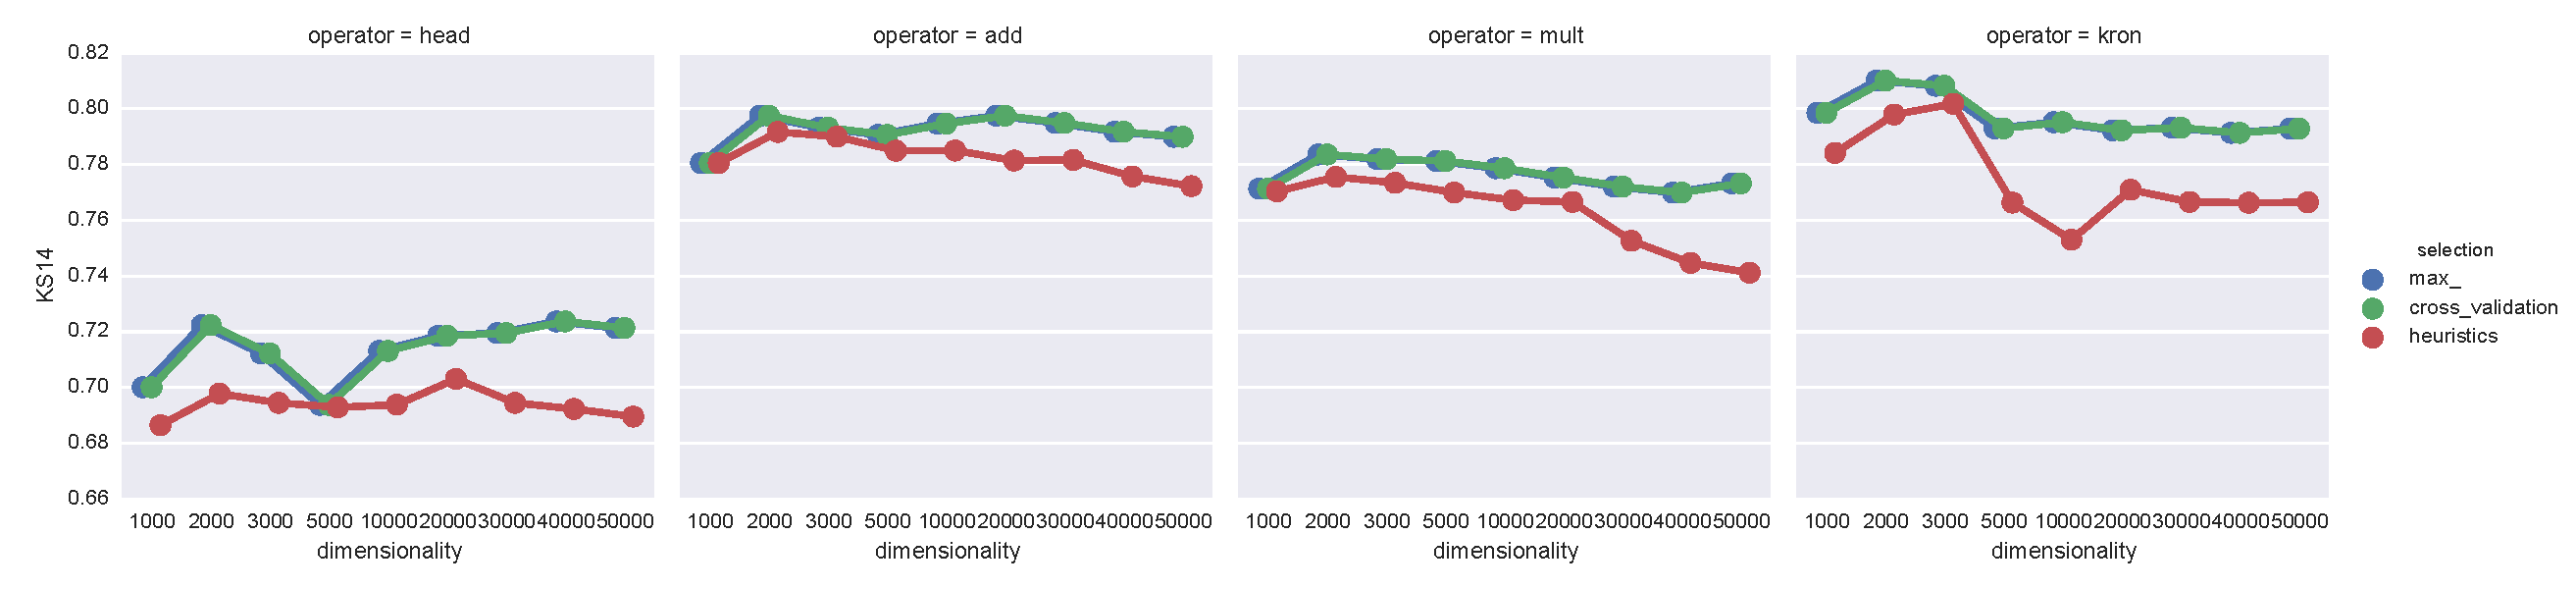
\includegraphics[width=\textwidth]{supplement/figures/ks14-results}
  \caption{KS14 results.}
  \label{fig:ks14-results}
\end{figure}

%%% Local Variables:
%%% mode: latex
%%% TeX-master: "../thesis"
%%% End:


Parameters of the baseline compositional method \texttt{head} are similar to the lexical Max selection (Table~\ref{tab:lexical-max-selection}), with an exception of \texttt{neg}, which controls vector sparsity, where higher values that are similar to MEN (Table~\ref{tab:men-max-selection}) are chosen.

All compositional operators agree in the choice of \texttt{freq} ($\log n$), \texttt{discr} (SCPMI) and similarity (correlation---note that Kronecker was tested only with the inner product for $D > 3\,000$ because of limited computational resources).

Compositional operators perform best with constant \texttt{freq} of 1, in contrast to the lexical setting, where $\log n$ is more beneficial. This might be because during composition the $\log n$ term dominates over the PMI value and minimises its effect.

Local context probabilities perform better in compositional tasks than in lexical tasks. Multiplication benefits from the unsmoothed distribution probability, while high-dimensional models perform best with smoothing ($\alpha = 0.75$), supporting H\ref{hyp:cds} that context smoothing is needed only for high-dimensional models. The only exceptions are additive models with $D < 5\,000$, where global probabilities perform best.

For low-dimensional spaces, addition performs best with sparse spaces ($k > 1$, $D < 5\,000$), but for high-dimensional spaces, addition performs best  with dense spaces ($k = 0,7$, $D \geq 5\,000$). This is against H\ref{hyp:neg} that states the opposite.

Multiplication, independently of dimensionality, performs best with dense spaces ($k = 0.2$).

Kronecker---in contrast to addition---performs best with dense low-dimensional models ($k = 0.2$, $D < 5\,000$) and sparser high-dimensional models ($k = 0.7$, $D \geq 5\,000$), which complies with H\ref{hyp:neg}. However, this difference might be explained by the change of the similarity measure, which is the inner product for $D \geq 5\,000$.

\subsection{Heuristics}
\label{sec:heuristics}

\begin{wraptable}[11]{O}{0.5\textwidth}
  %\vspace{-10pt}
  \centering

  \begin{tabular}{lr}
\toprule
      parameter &  partial $R^2$ \\
\midrule
            neg &  0.331 \\
           freq &  0.307 \\
       operator &  0.305 \\
            cds &  0.136 \\
     similarity &  0.061 \\
          discr &  0.054 \\
 dimensionality &  0.034 \\
\bottomrule
\end{tabular}


  \caption{KS14 feature ablation}
  \label{tab:ks14-ablation}
\end{wraptable}


The linear model achieves an $R^2$ of 0.794. The partial $R^2$s are shown in Table~\ref{tab:ks14-ablation}. The most influential parameters are \texttt{neg}, \texttt{freq}, compositional operator and \texttt{cds}. Interestingly, similarity has much less influence on this compositional dataset than on lexical datasets, where for Sim-Lex-999 (Table~\ref{tab:SimLex999-ablation}) and combined (Table~\ref{tab:lexical-ablation}) it is the most influential parameter. Also, note that dimensionality has the lowest partial $R^2$.

\subsubsection{Shifting}

For the baseline operator \texttt{head}, the best shifting choice of $k$ is 1 for spaces with dimensionality less than 5\,000 (Figure~\ref{fig:ks14-neg}). For $5\,000 \leq D < 30\,000$, \texttt{head} behaves best with $k = 1.4$. For $D \geq 3\,000$, $k$ should be set to 2.

For addition, spaces with $D < 20\,000$ should be used with $k = 1.4$, and with $k = 2$ otherwise.

For multiplication, there are three most beneficial choices: for $D < 10\,000$ $k = 0.5$, for $10\,000 \leq D < 30\,000$ $k = 0.7$ and, finally, for $D > 30\,000$ $k = 1$.

Kronecker shows a behaviour  similar to multiplication for $k$ as dimensionality increases, but prefers sparser spaces. For $D < 3\,000$: $k = 0.5$, for $3\,000 \leq D < 20\,000$: $k = 0.7$ and for $20\,000 \leq D$: $k = 1$.

All operators behave in accordance to H\ref{hyp:neg} that low-dimensional spaces benefit from being dense, while high-dimensional spaces benefit from being sparse.

\begin{figure}
% \begin{wrapfigure}{O}{0.5\textwidth}
  % \vspace{-30pt}
  \centering

  \begin{subfigure}[t]{\textwidth}
    \includegraphics[width=1.1\textwidth]{supplement/figures/ks14-interaction-neg}

  \caption{\texttt{neg}}
  \label{fig:ks14-neg}
  \end{subfigure}

  \begin{subfigure}[t]{\textwidth}
    \includegraphics[width=1.1\textwidth]{supplement/figures/ks14-interaction-freq}

  \caption{\texttt{freq}}
  \label{fig:ks14-freq}
  \end{subfigure}

  \caption{KS14.}
\end{figure}


\subsubsection{Frequency}
The best option of frequency for the baseline operator \texttt{head} is $\log n$ (Figure~\ref{fig:ks14-freq}). The constant frequency 1 is very close to $\log n$, but its performance declines for spaces with $D > 20\,000$.

For addition, frequency should be set to 1 for spaces with $D < 5\,000$ and to $\log n$ otherwise.

There is one choice of frequency for multiplication: 1. However, $\log n$ behaves similarly to it when $D \geq 3\,000$.

Kronecker follows addition with regard to frequency, but the split point is $D = 10\,000$: low-dimensional spaces should be used with constant frequency 1, and high-dimensional spaces with $\log n$.

Generally, H\ref{hyp:freq}---that non-constant frequency is beneficial for high-dimensional spaces---is supported by all operators in this dataset.

\subsubsection{Context distribution smoothing}

\begin{figure}
% \begin{wrapfigure}{O}{0.5\textwidth}
  % \vspace{-30pt}
  \centering

  \begin{subfigure}[t]{\textwidth}
    \includegraphics[width=1.1\textwidth]{supplement/figures/ks14-interaction-cds}

  \caption{\texttt{cds}}
  \label{fig:ks14-cds}
  \end{subfigure}

  \begin{subfigure}[t]{\textwidth}
    \includegraphics[width=1.1\textwidth]{supplement/figures/ks14-interaction-similarity}

  \caption{\texttt{similarity}}
  \label{fig:ks14-similarity}
  \end{subfigure}

  \caption{KS14.}
\end{figure}

The baseline operator \texttt{head} with spaces with dimensionality less than 20\,000 should be used with global probabilities, and more dimensional models should be used with smoothed, local probabilities: $\alpha = 0.75$ (Figure~\ref{fig:ks14-cds}).

All other operators perform best with global context probability. Even though local context probability with $\alpha = 1$ is close to global, H\ref{hyp:cds} is not supported by this dataset: context distribution smoothing does not affect high-dimensional spaces.

\subsubsection{Similarity}
The baseline operator \texttt{head} on spaces with $D < 20\,000$ performs best with cosine similarity, while more dimensional models prefer correlation as the similarity measure (Figure~\ref{fig:ks14-similarity}), strictly according to H\ref{hyp:similarity}: the adjustment by the mean value that is performed by correlation is need by high-dimensional models.

Other operators work best with correlation. Addition and multiplication also support H\ref{hyp:similarity} that correlation is beneficial in high-dimensional spaces. In the case of multiplication, correlation dominates over cosine, even for small values of $D$. There is little to say about Kronecker, as it is tested only with the inner product for spaces with $D > 3\,000$, due to its computational complexity ($\mathcal{O}(n^2)$ with respect to the number of vector components).

\subsubsection{Discriminativeness}

\begin{figure}[b]
% \begin{wrapfigure}{O}{0.5\textwidth}
  % \vspace{-30pt}
  \centering

  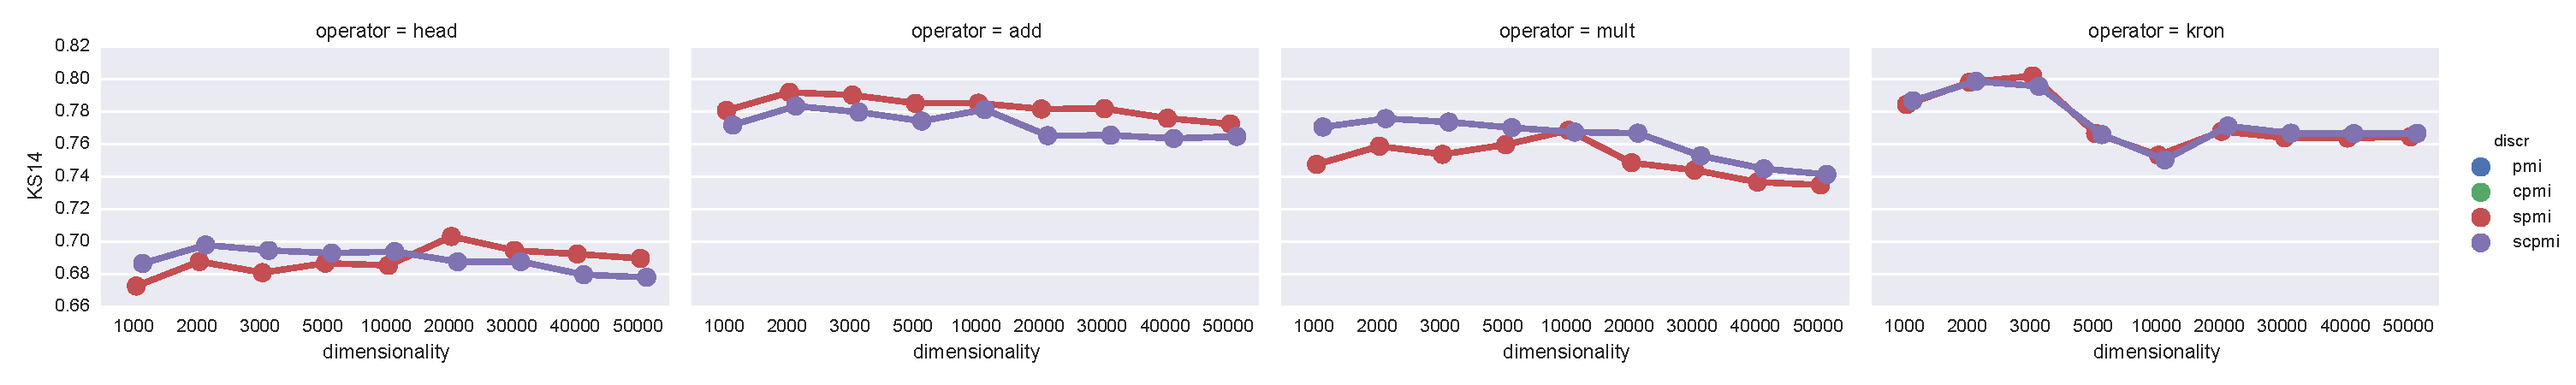
\includegraphics[width=1.1\textwidth]{supplement/figures/KS14-interaction-discr}

  \caption{KS14 influence of \texttt{discr}}
  \label{fig:ks14-discr}
\end{figure}

The baseline operator \texttt{head} with $D < 20\,000$ prefers SCPMI as the discriminativeness weighting. SPMI is preferred otherwise (Figure~\ref{fig:ks14-discr}).

For addition, SPMI is the better choice. For multiplication, SCPMI is more beneficial, as expected by H\ref{hyp:comp-pmi-cpmi}: the compression of PMI values improves the performance of compositional models.

For Kronecker, the two choices are very close to each other. For spaces with dimensionality less than 20\,000, SPMI is slightly better; for spaces with greater dimensionality---SCPMI.

\subsection{Difference between Max selection and heuristics on KS14}

Table~\ref{tab:ks14-heuristics-selection} shows the selection based on heuristics, which is more homogeneous than the selection based on the highest score (Table~\ref{tab:ks14-max-selection}). Both methods agree on the similarity choice (with the exception of \texttt{head}).

Multiplication agrees on the majority of parameters, except \texttt{cds} and \texttt{neg}. Local probabilities ($\alpha = 1$) and $k = 0.2$ give the highest score, while manual selection picked global context probabilities with \texttt{neg} in the range of 0.5 to 1, in accordance with H\ref{hyp:neg} that high-dimensional spaces should be sparser.

The average difference between Max and heuristic-based selections is 0.022. Per operator, the differences are: 0.028 (\texttt{head}), 0.012 (addition), 0.018 (multiplication) and 0.028 (Kronecker). All values are within the 10\% set by H\ref{hyp:10percent}.

\section{Experiments on GS11 dataset}
\label{sec:gs11}

GS11 is a dataset of transitive sentences \cite{Grefenstette:2011:ESC:2145432.2145580,Grefenstette:2011:ETV:2140490.2140497}. It consists of ambiguous transitive verbs together with their arguments and two landmark verbs that each disambiguate a particulate sense of the ambiguous verb. Human judgements provide pairwise similarity scores between the sentence with the ambiguous verb and the two sentences with the landmark verbs.

\subsection{Max selection}
\label{sec:max-selection-gs11}

\begin{figure}[b]
  \centering

    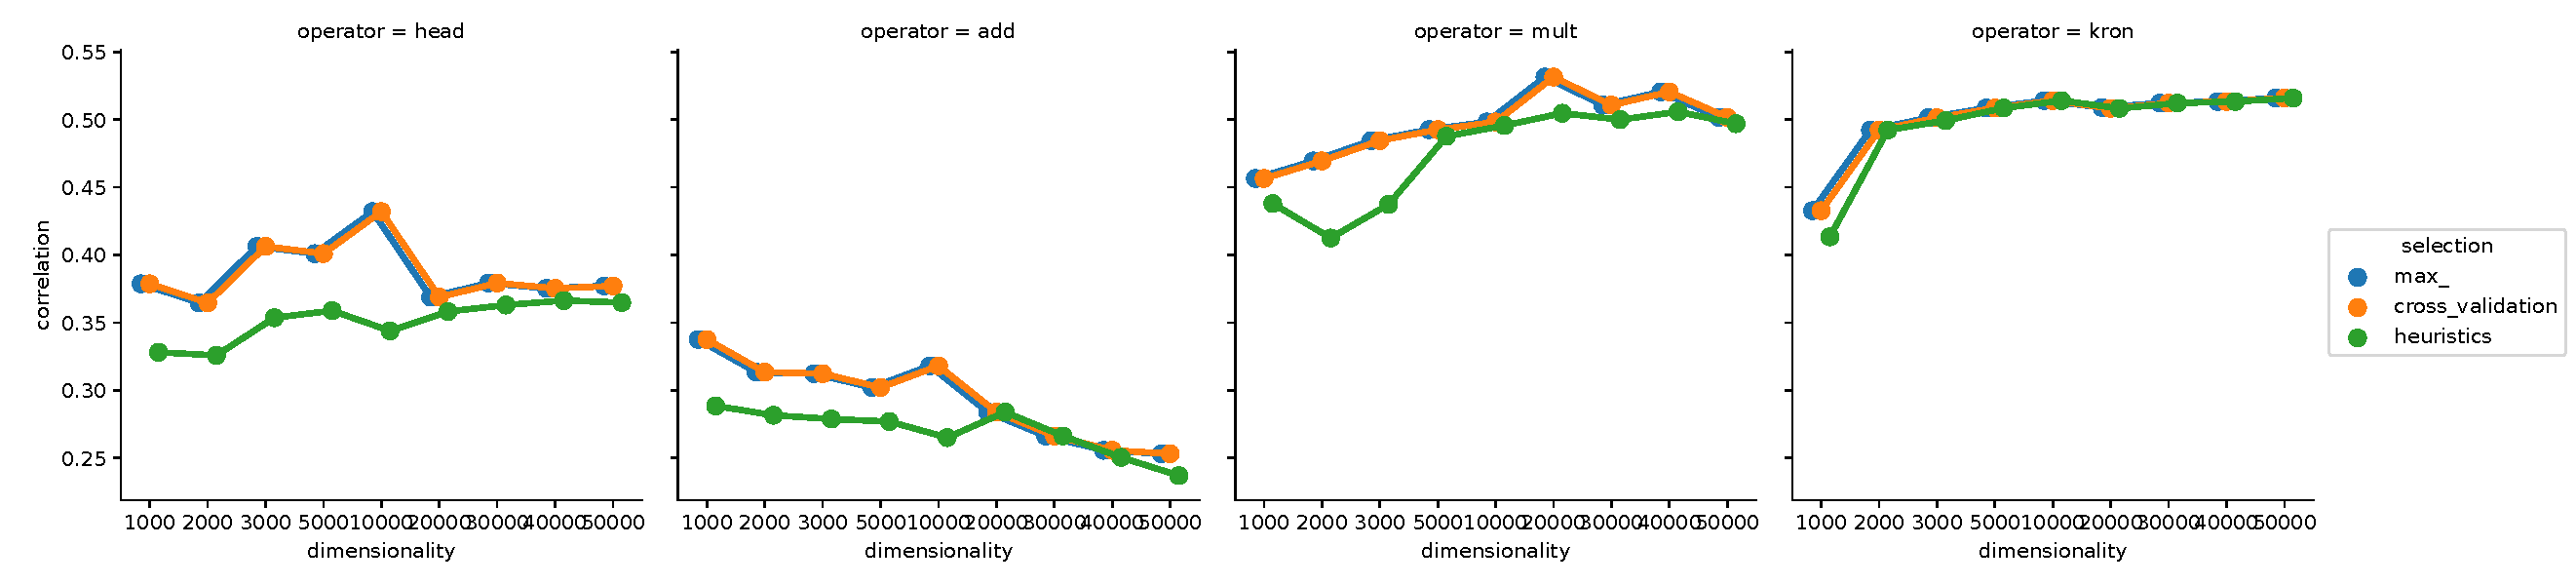
\includegraphics[width=\textwidth]{supplement/figures/gs11-results}
  \caption{GS11 results.}
  \label{fig:gs14-results}
\end{figure}

%%% Local Variables:
%%% mode: latex
%%% TeX-master: "../thesis"
%%% End:


Figure~\ref{fig:gs14-results} shows performance of the compositional models on the verb disambiguation task. Table~\ref{tab:gs11-max-selection} shows the selected model performance together with chosen parameters.

Multiplication with 20\,000 dimensions gives the highest result of 0.532. Kronecker gets close with a score of 0.516 with $D = 50\,000$, giving no support to H\ref{hyp:order} that word order is important for similarity measurement. Addition does not outperform the baseline \texttt{head} operator: addition scores 0.338, while \texttt{head}'s best performance is 0.432.

The behaviour of the baseline operator \texttt{head} is unstable for dimensions less than 20\,000, and its best behaviour might be the case of overfitting similarly with SimLex-999. However, models with dimensions greater than 20\,000 yield similar scores, even though the parameters are different.

In general, Max parameter selection is very different than the one based on KS14 (Table~\ref{tab:ks14-max-selection}). Compositional operators behave best with $\log n$ frequency, especially Kronecker. PMI often outperforms other discriminativeness components in the case of \texttt{head} and addition. Global context probability estimation behaves better than local and correlation is not always the best similarity measure.

Addition's behaviour degrades as dimensionality increases, whereas multiplication's behaviour increases, but becomes unstable for spaces with more than 20\,000 dimensions. Kronecker depends on the dimensionality the least.

Addition works best with dense models. Multiplication and Kronecker prefer dense, low-dimensional spaces and sparse, high-dimensional spaces, supporting H\ref{hyp:neg} that a frequency component is required for high-dimensional spaces.

\subsection{Heuristics}
\label{sec:heuristics-gs11}

The linear model achieves an $R^2$ of 0.753. The partial $R^2$ scores are shown in Table~\ref{tab:gs11-ablation}. The most influential parameters are a compositional operator, \texttt{freq} and \texttt{neg}. This is the same as in the case of KS14, but in reverse order (Table~\ref{tab:ks14-ablation}).

\subsubsection{Frequency}

\begin{wraptable}[8]{O}{0.5\textwidth}
% \begin{table}[b]
  \vspace{-4em}
  \centering
  \begin{tabular}{lr}
\toprule
      parameter &  partial $R^2$ \\
\midrule
       operator &  0.37 \\
           freq &  0.21 \\
            neg &  0.18 \\
     similarity &  0.09 \\
            cds &  0.05 \\
          discr &  0.04 \\
 dimensionality &  0.04 \\
\bottomrule
\end{tabular}


  \caption{GS11 feature ablation}
  \label{tab:gs11-ablation}
\end{wraptable}

On average, $\log n$ behaves best for all operators (Figure~\ref{fig:gs11-freq}). For $D \leq 5\,000$, 1 is also a good frequency choice, supporting H\ref{hyp:freq} that non-constant frequency component is required for high-dimensional spaces.

\subsubsection{Shifting}

The baseline operator \texttt{head} on average works best with shifted models. For models with dimensionality less than 3\,000, $k = 0.5$ is best, otherwise $k = 0.7$ is more beneficial (Figure~\ref{fig:gs11-neg}).

For addition, models without shifting behave best for $D < 20\,000$, however, for more dimensional spaces, $k = 0.2$ should be preferred. This is a weak support of H\ref{hyp:neg} (high-dimensional vectors should be sparse) because unshifted spaces can be seen as shifted with a very small $\alpha$ value.

Multiplication also works best with unshifted low-dimensional spaces ($D < 5\,000$) and with $k = 0.7$ for high-dimensional spaces, supporting H\ref{hyp:neg}.

Kronecker prefers shifting. For spaces with dimensionality less than 20\,000 $k = 0.7$ and $k = 1$ otherwise. This is inline with H\ref{hyp:neg}.

\begin{figure}
% \begin{wrapfigure}{O}{0.5\textwidth}
  % \vspace{-30pt}
  \centering

  \begin{subfigure}[t]{\textwidth}
    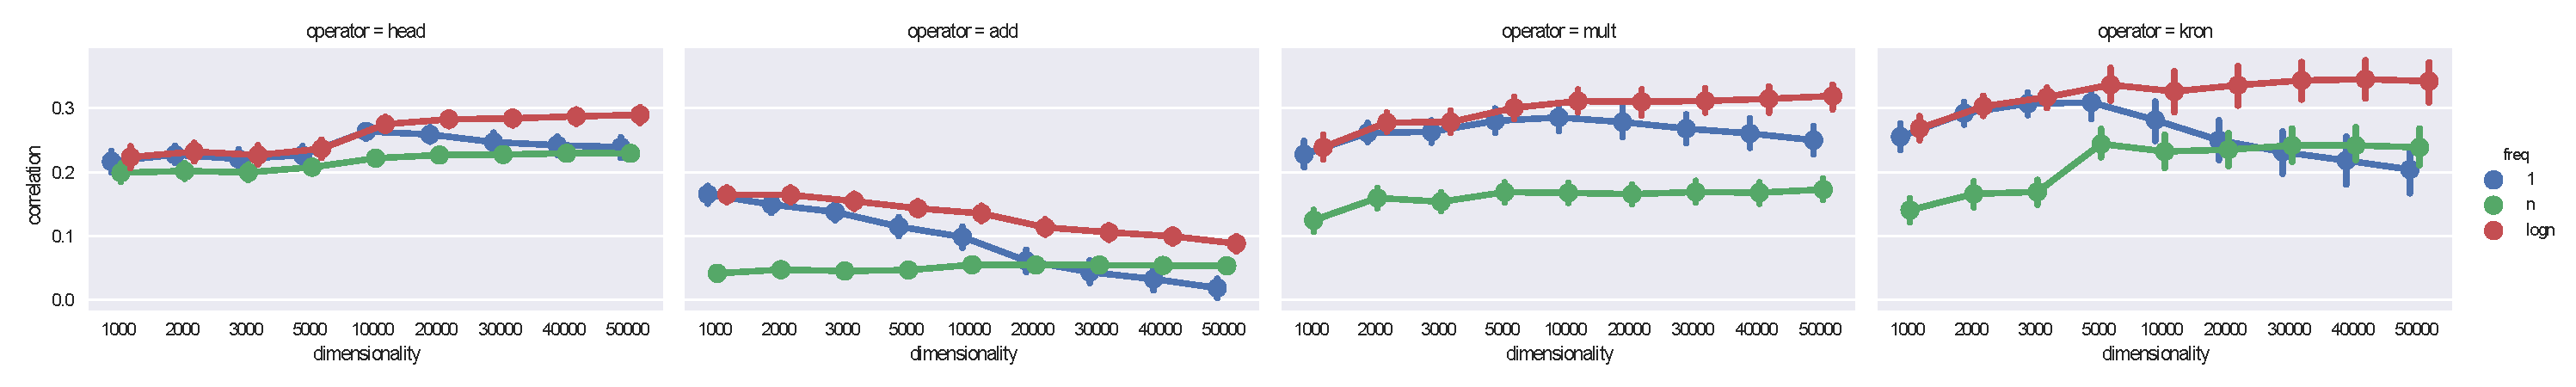
\includegraphics[width=1.1\textwidth]{supplement/figures/GS11-interaction-freq}

  \caption{\texttt{freq}}
  \label{fig:gs11-freq}
  \end{subfigure}

  \begin{subfigure}[t]{\textwidth}
    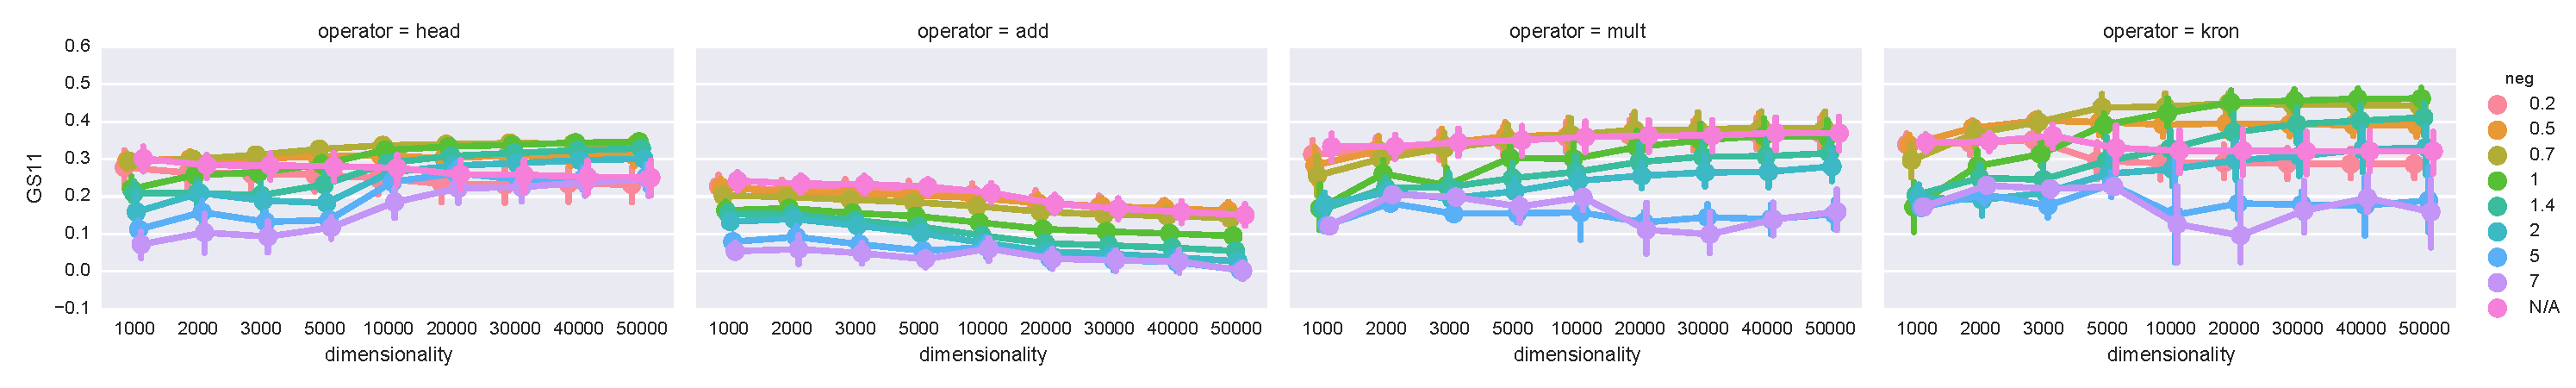
\includegraphics[width=1.1\textwidth]{supplement/figures/GS11-interaction-neg}

  \caption{\texttt{neg}}
  \label{fig:gs11-neg}
  \end{subfigure}

  \caption{GS11 influence of \texttt{freq} and \texttt{neg}}
\end{figure}


\subsubsection{Similarity}

The baseline operator \texttt{head} and multiplication work best with cosine similarity, addition with correlation and Kronecker with inner product (Figure~\ref{fig:gs11-similarity}).

Addition strictly supports H\ref{hyp:similarity} that cosine is optimal for high-dimensional spaces, while multiplication supports it by behaving similarly to cosine and correlation.

\subsubsection{Context distribution smoothing}

The baseline operator \texttt{head} with $D < 10\,000$ works best with global context probabilities. For more dimensional spaces, local context probabilities $\alpha = 1$ should be preferred (Figure~\ref{fig:gs11-cds}).

Addition works best with local probabilities. In the low-dimensional case, when $D < 20\,000$, unsmoothed estimation ($\alpha = 1$) is preferred and $\alpha = 0.75$ should be chosen otherwise.

Multiplication works best with global context probabilities and Kronecker with smoothed local ($\alpha = 0.75$).

There is no support of H\ref{hyp:cds} (context distribution smoothing leads to optimal results with high-dimensional models) because global context probabilities outperform other choices for multiplication, addition behaves the same with all options and Kronecker works best with $\alpha = 0.75$.

\begin{figure}
% \begin{wrapfigure}{O}{0.5\textwidth}
  % \vspace{-30pt}
  \centering

  \begin{subfigure}[t]{\textwidth}
    \includegraphics[width=1.1\textwidth]{supplement/figures/gs11-interaction-similarity}

  \caption{Similarity}
  \label{fig:gs11-similarity}
  \end{subfigure}

  \begin{subfigure}[t]{\textwidth}
    \includegraphics[width=1.1\textwidth]{supplement/figures/gs11-interaction-cds}

  \caption{\texttt{cds}}
  \label{fig:gs11-cds}
  \end{subfigure}

  \caption{GS11.}
\end{figure}


\subsubsection{Discriminativeness}

\begin{figure}[b]
% \begin{wrapfigure}{O}{0.5\textwidth}
  % \vspace{-30pt}
  \centering

  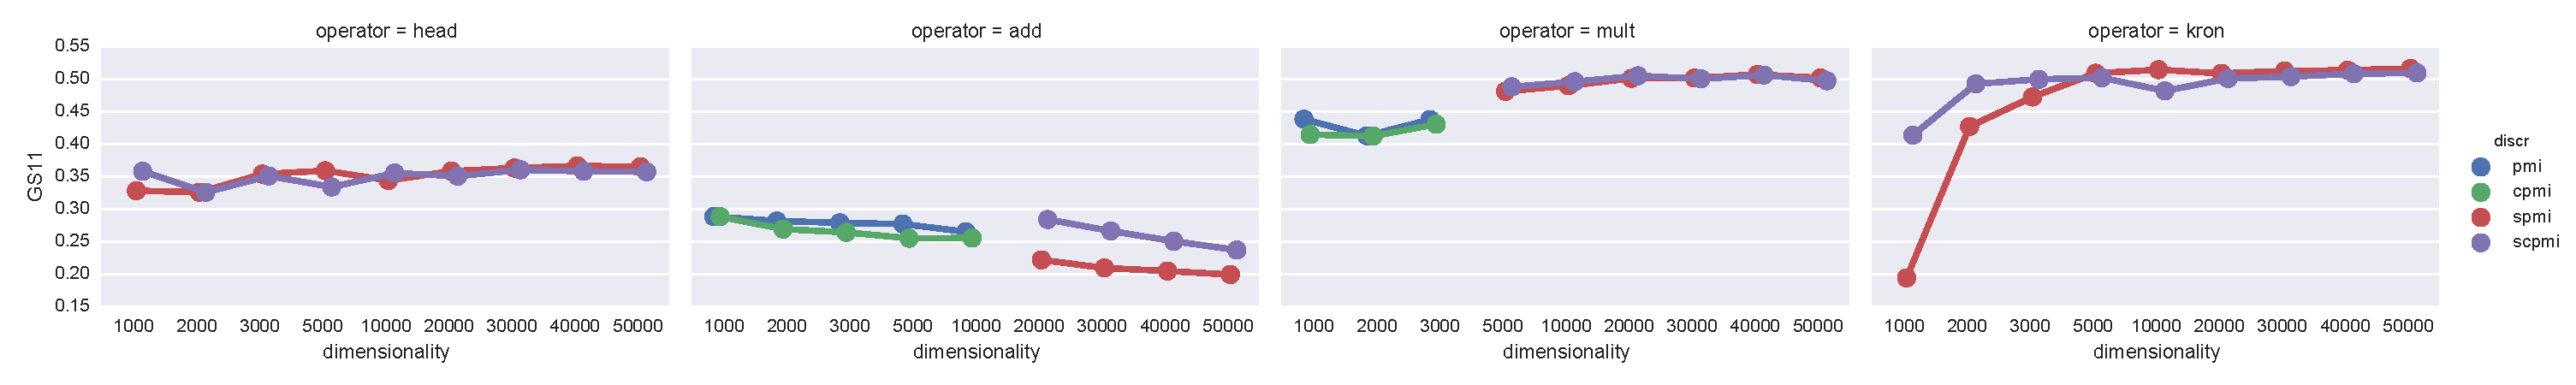
\includegraphics[width=1.1\textwidth]{supplement/figures/GS11-interaction-discr}

  \caption{GS11 \texttt{discr}}
  \label{fig:gs11-discr}
\end{figure}


The baseline operator \texttt{head} works best with SPMI, but SCPMI is very close (Figure~\ref{fig:gs11-discr}). Addition works best with PMI for $D < 20\,000$ and SCPMI otherwise.

Multiplication is similar to addition in that it prefers PMI in the low-dimensional case and SCPMI in the high-dimensional case, but the change happens at 5\,000 dimensions rather than 20\,000.

Kronecker with less than 5\,000 dimensions prefers SCPMI and SPMI, which is opposite to addition and multiplication.

This dataset does not give evidence to support H\ref{hyp:comp-pmi-cpmi}---PMI values should be compressed when used in compositional setting---because there is almost no difference between *PMI and *CPMI.

\subsection{Difference between Max selection and heuristics on GS11}

Only logarithmic frequency component ($\log n$) was chosen by heuristics (Table~\ref{tab:gs11-heuristics-selection}), while there is a mix of 1 and $\log n$ in the Max selection (Table~\ref{tab:gs11-max-selection}).

Kronecker and most of multiplication's discriminativeness choices agree, while for \texttt{head} and addition there is little agreement between parameter selection. The same goes for context distribution smoothing and shifting.

Similarity choice is the same for Kronecker and addition, but \texttt{head} and multiplication---according to heuristics---should be used with cosine similarity, while there is no single metric that leads to maximum performance.

The overall average normalised difference in results between Max and heuristic-based selections is 0.054. Per operator, the differences are: 0.090 \texttt{head}, 0.077 addition, 0.043 multiplication and 0.006 Kronecker. All the values are within the 10\% boundary set by H\ref{hyp:10percent}.

\section{Experiments on PhraseRel dataset}
\label{sec:phraserel-experiment}

PhraseRel is a dataset that is built for evaluation of distributional models, but instead of similarity judgements, relevance judgements are provided. The evaluation measure is relevance@3. This is the proportion of the retrieval results for which there is a relevant document among the top three ranked documents.

\subsection{Max selection}
\label{sec:max-selection-phraserel}

\begin{figure}
  \centering

    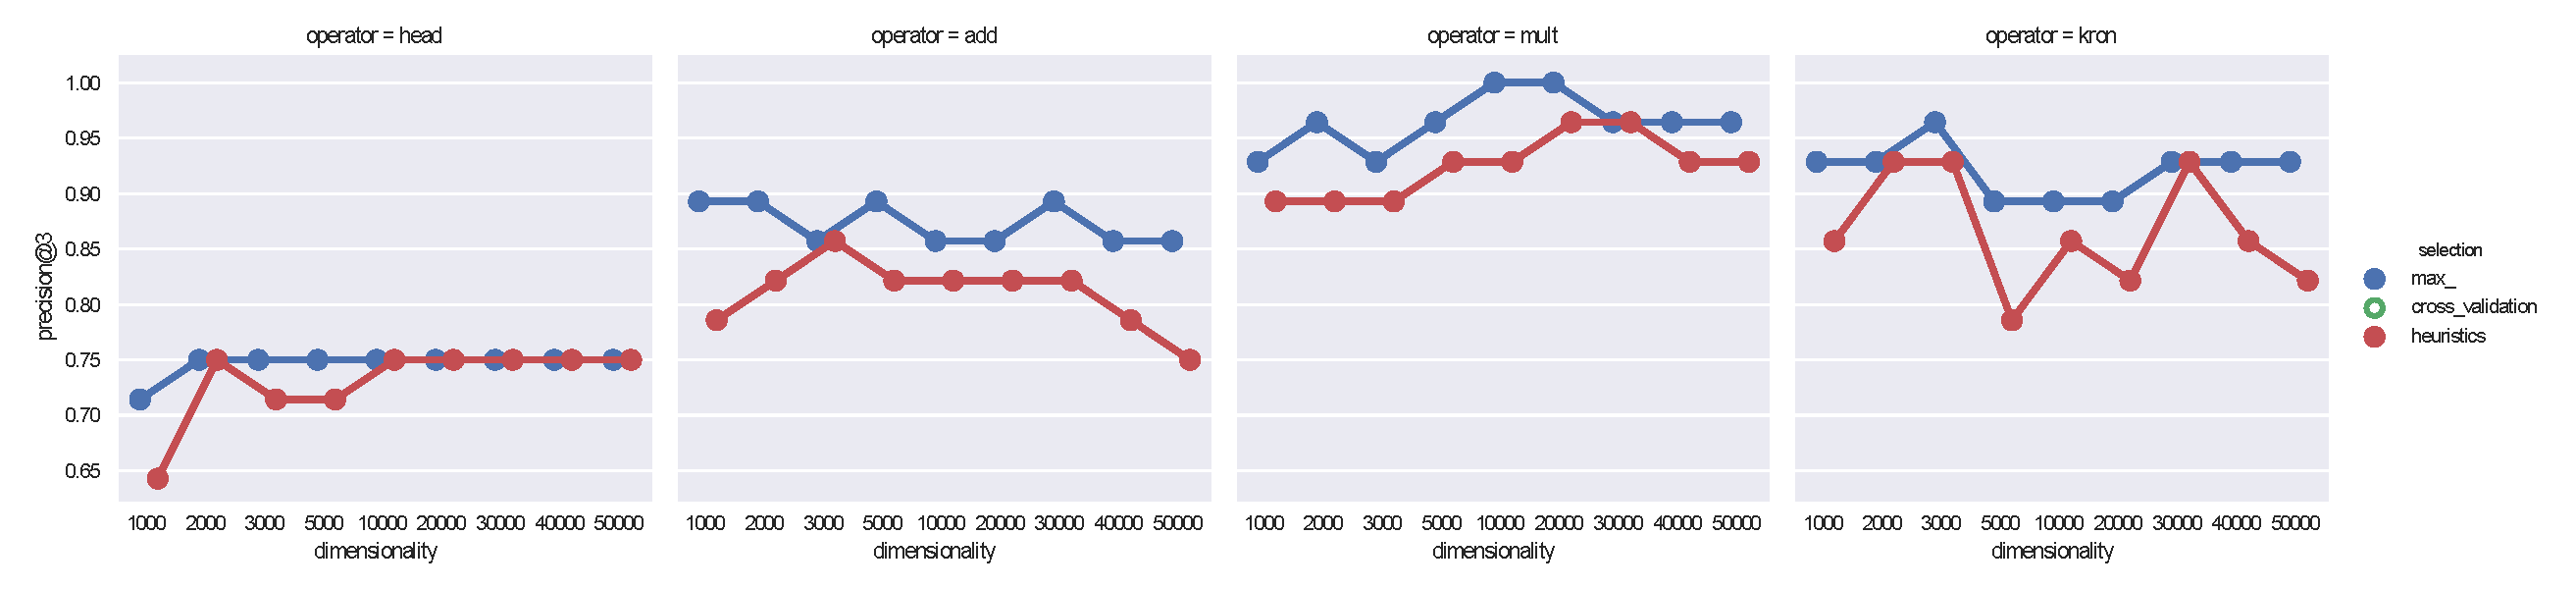
\includegraphics[width=\textwidth]{supplement/figures/phraserel-results}
  \caption{PhraseRel results.}
  \label{fig:phraserel-results}
\end{figure}

%%% Local Variables:
%%% mode: latex
%%% TeX-master: "../thesis"
%%% End:


Figure~\ref{fig:phraserel-results} shows the performance of the models on the PhraseRel dataset. All operators outperform the non-compositional \texttt{head} baseline. Table~\ref{tab:phraserel-max-selection} shows the models that yield the best result together with model parameters.

Multiplication, in general, outperforms all other operators, and with the dimensions of 10\,000 and 20\,000, gets the perfect score of 1. The fact that Kronecker (a word order sensitive operator) is outperformed by multiplication (a word order insensitive operator) gives no support of H\ref{hyp:order} that word order matters. Model performance weakly depends on the dimensionality for all operators. Multiplication and Kronecker show strong performance similarly to the preliminary study, where similarity was assumed to correspond to relevance \cite{Milajevs:2015:IMN:2808194.2809448}.

Addition and Kronecker achieve the best score with constant frequency, \texttt{head} works best with linear frequency and multiplication with sublinear ($\log n$) frequency.

SPMI is the preferred discriminativeness component for the low-dimensional spaces ($D < 10\,000$) for the baseline \texttt{head}, otherwise, SCPMI is the best behaving \texttt{discr}. For addition and the spaces with $D > 1\,000$, SPMI is the best, while for the spaces with the same dimensionality, multiplication prefers CPMI, which is in line with H\ref{hyp:comp-pmi-cpmi}: PMI values should be compressed when used in compositional tasks. Kronecker, most of the time, prefers SCPMI.

The baseline operator \texttt{head} with dimensions less than 20\,000 works best with local smoothed context probabilities, however, for more dimensional spaces, global context probabilities are more competitive. On the contrary, addition prefers smoothed local context probabilities for spaces with dimensions more than 5\,000. Multiplication exhibits different pattern: when a model contains few dimensions, it prefers local, smoothed context probabilities, and for high-dimensional spaces it prefers local, but unsmoothed context probabilities, which goes against H\ref{hyp:cds} (context distribution smoothing should be optimal with high-dimensional spaces). Kronecker is inconsistent with regards to the choice of \texttt{cds}, but for models with $D \geq 30\,000$, global context probabilities perform the best.

Regarding shifting, the baseline operator \texttt{head} prefers sparse spaces $k > 1$, but as dimensionality increases, the optimal $k$ values decrease. Addition does not show a consistent behaviour with regard to this parameter. Multiplication, in general, benefits from dense, unshifted spaces. Kronecker works best with sparse spaces with increasing sparsity as the dimensionality increases, supporting H\ref{hyp:neg}: low-dimensional models should be dense, but high-dimensional models should be sparse.

The baseline operator \texttt{head} benefits from the correlation as the similarity measure, as does multiplication. Addition works best with correlation with spaces $D < 10\,000$, and with the inner product for more dimensional spaces. Multiplication works best with correlation. Kronecker, for spaces with less than 5\,000 dimensions, works best with correlation and with the inner product, otherwise.

\subsection{Heuristics}
\label{sec:heuristics-phraserel}

\begin{wraptable}[10]{O}{0.5\textwidth}
% \begin{table}[b]
  \vspace{-1em}
  \centering

  \begin{tabular}{lr}
\toprule
      parameter &  partial $R^2$ \\
\midrule
            neg &       0.58 \\
       operator &       0.35 \\
            cds &       0.08 \\
           freq &       0.04 \\
     similarity &       0.03 \\
 dimensionality &       0.03 \\
          discr &       0.02 \\
\bottomrule
\end{tabular}


  \caption{PhraseRel feature ablation}
  \label{tab:phraserel-ablation}
\end{wraptable}


The linear model achieves an $R^2$ of 0.822. The partial $R^2$ scores are shown in Table~\ref{tab:phraserel-ablation}. The most influential parameters are \texttt{neg}, operator and \texttt{cds}, but the first two have partial $R^2$ scores much higher than the other parameters. Table~\ref{tab:phraserel-heuristics-selection} shows the performance of the chosen models.

\subsubsection{Shifting}
\label{sec:shifting-phraserel}

The baseline operator \texttt{head} should be used with $k = 1.4$, addition should be used with $k = 2$ and multiplication should be used with $k = 0.5$ (Figure~\ref{fig:phraserel-neg}).

Kronecker has three optimal values of $k$ that are proportional to dimensionality. For models with dimensionality less than 5\,000, $k = 0.5$ is preferred; for $5\,000 \leq D < 20\,000$, the most beneficial choice of \texttt{neg} is $k = 1$; finally, for spaces with more than 20\,000 dimensions, $k$ should be set to 1.4. This supports H\ref{hyp:neg} that model sparsity should increase as dimensionality increases.

\begin{figure}
% \begin{wrapfigure}{O}{0.5\textwidth}
  % \vspace{-30pt}
  \centering

  \begin{subfigure}[t]{\textwidth}
    \includegraphics[width=1.1\textwidth]{supplement/figures/phraserel-interaction-neg}

  \caption{\texttt{neg}}
  \label{fig:phraserel-neg}
  \end{subfigure}

  \begin{subfigure}[t]{\textwidth}
    \includegraphics[width=1.1\textwidth]{supplement/figures/phraserel-interaction-cds}

  \caption{\texttt{cds}}
  \label{fig:phraserel-cds}
  \end{subfigure}

  \caption{PhraseRel.}
\end{figure}


\subsubsection{Context distribution smoothing}
\label{sec:cont-distr-smooth-phraserel}

The best choice for the baseline operator \texttt{head} deponds on dimensionality: spaces with less than 10\,000 dimensions benefit from smoothed local context probabilities ($\alpha = 0.75$, Figure~\ref{fig:phraserel-cds}). Addition and multiplication work best with global context probabilities, while Kronecker prefers unsmoothed local probabilities ($\alpha = 1$).

\subsubsection{Frequency}
\label{sec:frequency-phraserel}

The baseline operator\texttt{head} works best with linear frequency, but the difference between other options is small (Figure~\ref{fig:phraserel-freq}). Addition benefits from linear frequency, but sublinear frequency is very close. Multiplication works best with sublinear frequency, but linear is very close to it. Finally, Kronecker works best with $\log n$ with spaces with dimensionality less than 5\,000, and with linear frequency with more dimensional spaces.

In general, H\ref{hyp:freq} (non-linear frequency should be used with high-dimensional spaces) holds, because there is no difference between 1 and $\log n$ choices in model performance.

\begin{figure}[b]
% \begin{wrapfigure}{O}{0.5\textwidth}
  % \vspace{-30pt}
  \centering

  \begin{subfigure}[t]{\textwidth}
    \includegraphics[width=1.1\textwidth]{supplement/figures/phraserel-interaction-freq}

  \caption{\texttt{freq}}
  \label{fig:phraserel-freq}
  \end{subfigure}

  \begin{subfigure}[t]{\textwidth}
    \includegraphics[width=1.1\textwidth]{supplement/figures/phraserel-interaction-similarity}

  \caption{similarity}
  \label{fig:phraserel-similarity}
  \end{subfigure}

  \caption{PhraseRel.}
\end{figure}


\subsubsection{Similarity}
\label{sec:similarity-phraserel}

For all operators, there is little difference between cosine and correlation, weakly supporting H\ref{hyp:similarity} that correlation should be used with high-dimensional spaces and cosine with low-dimensional spaces.

The baseline operator \texttt{head} works best with correlation as the similarity measure with models with $D < 5\,000$, and with cosine for more dimensional ones (Figure~\ref{fig:phraserel-similarity}). Note, however, that the difference between the two is very small.

Addition benefits from cosine when $D < 20\,000$ and from inner product otherwise. But, in the case of addition, all three similarity measures are close to each other.

Multiplication works best with correlation. Where tested, correlation behaves best with Kronecker.

\subsubsection{Discriminativeness}
\label{sec:discriminativeness-phraserel}

\begin{figure}[b]
% \begin{wrapfigure}{O}{0.5\textwidth}
  % \vspace{-30pt}
  \centering

  \includegraphics[width=1.1\textwidth]{supplement/figures/phraserel-interaction-discr}

  \caption{PhraseRel \texttt{discr}}
  \label{fig:phraserel-discr}
\end{figure}


The baseline \texttt{head} prefers different discriminativeness components depending on dimensionality. For models with $D < 5\,000$, SPMI is the best, while for other dimensions SCPMI is more competitive.

Addition and Kronecker benefit from SPMI, and multiplication from SCPMI, apart from the dimensionality of 10\,000. H\ref{hyp:comp-pmi-cpmi}, that PMI compression improves results in compositional tasks, is only supported by multiplication.

\subsection{Difference between Max selection and heuristics on PhraseRel}
\label{sec:diff-phraserel}

Manual parameter selection is more stable than the one based on maximum values. However, in cases where different parameters are picked, there is little or no difference between these parameter choices. For example, studied similarity measures yield similar average performance for addition, see Figure~\ref{fig:phraserel-freq}.

Manual heuristics do not pick the best result of 1 (Table~\ref{tab:phraserel-max-selection}), but are close with a multiplicative model with 20\,000 and 30\,000 dimensions, yielding a score of 0.964 (Table~\ref{tab:phraserel-heuristics-selection}).

The average relative difference between the Max selection and the selection based on heuristics is 0.022 for \texttt{head}, 0.072 for addition, 0.041 for multiplication and 0.061 for Kronecker.

Over all compositional methods, the difference is 0.049, which is within the 10\% limit set by H\ref{hyp:10percent}.

\section{Selected model transfer across the datasets}
\label{sec:select-model-transf-comp}

\begin{figure}[t]
  \centering
    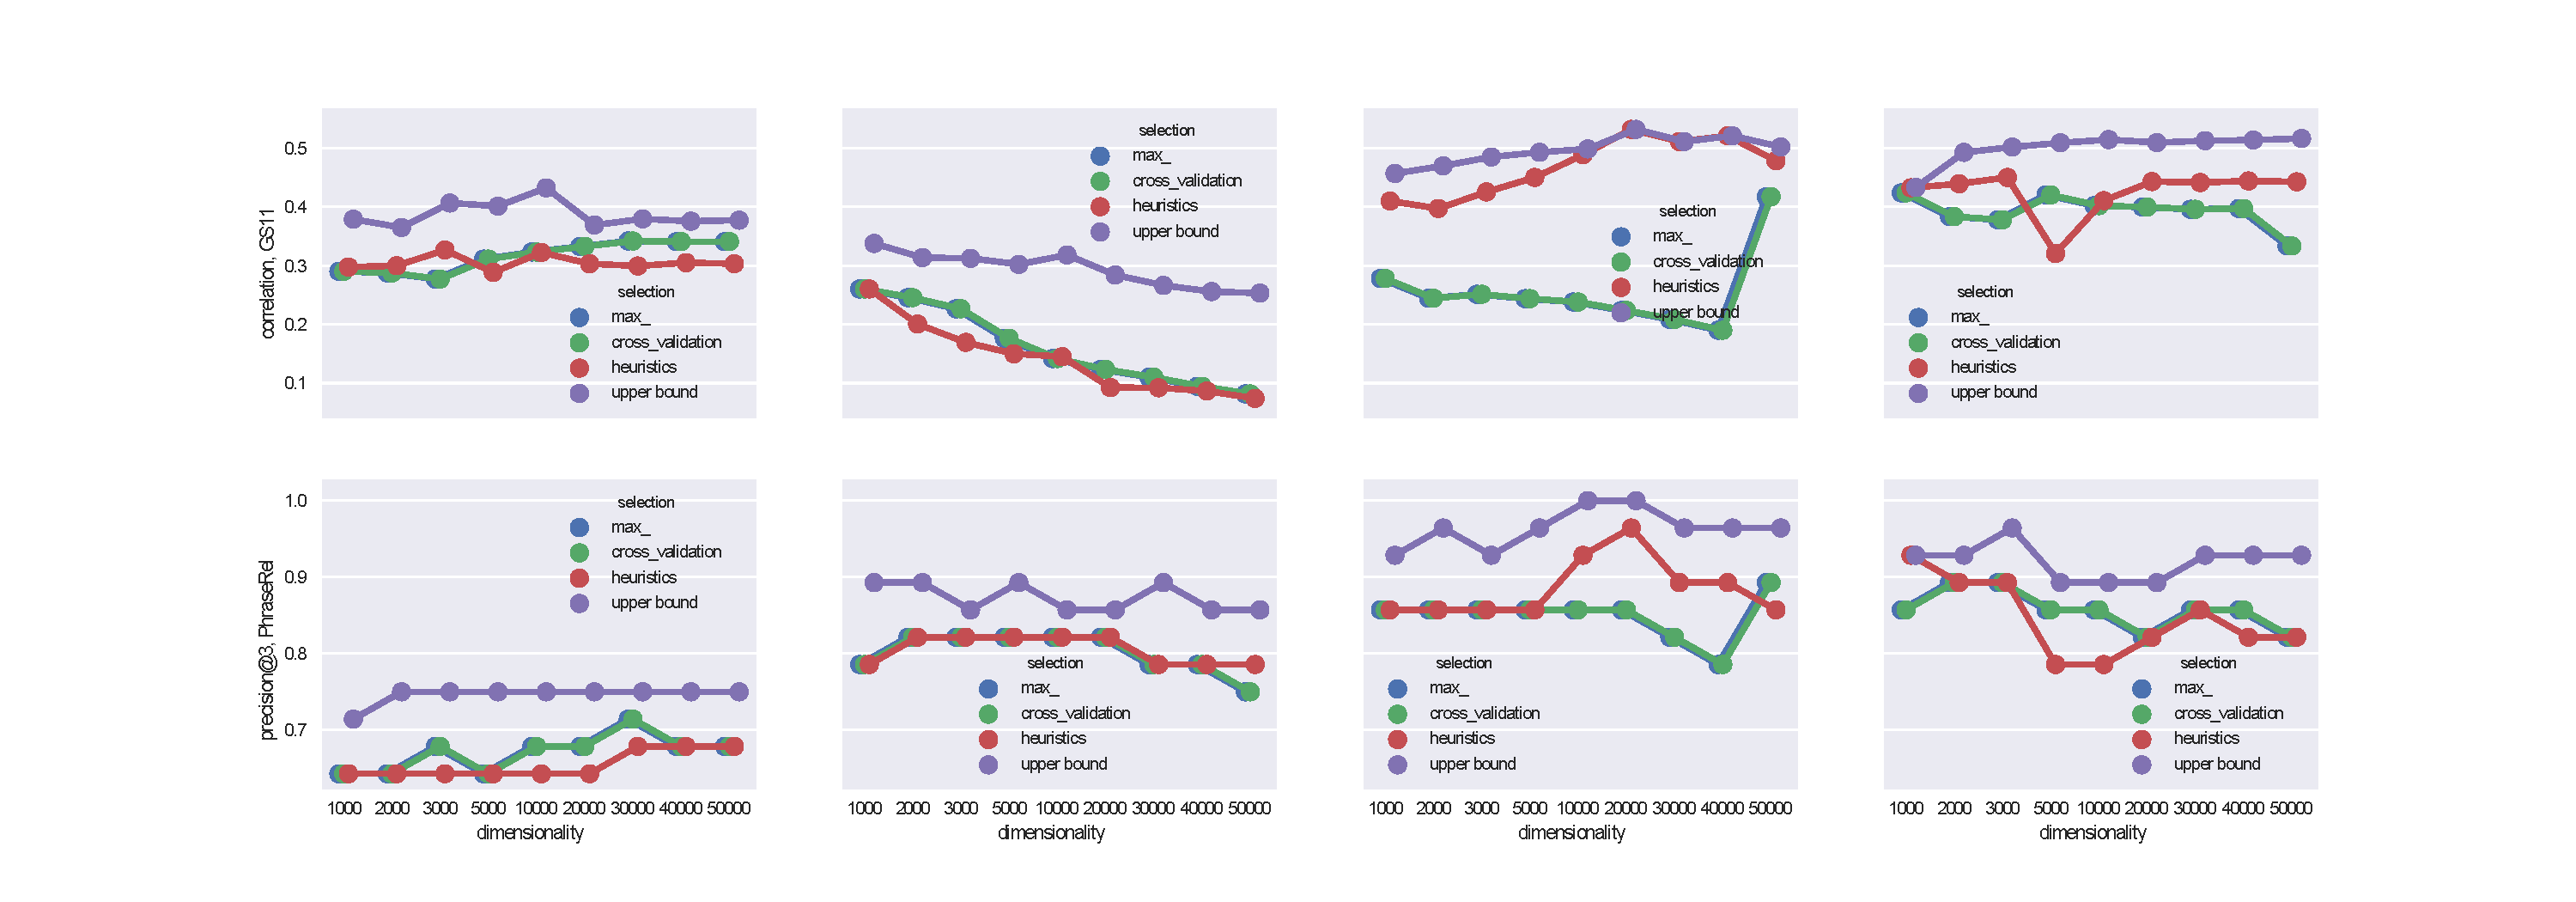
\includegraphics[width=\textwidth]{supplement/figures/KS14-transfer}
    \caption{Transfer from KS14.}
    \label{fig:ks14-transfer}
\end{figure}

%%% Local Variables:
%%% mode: latex
%%% TeX-master: "../thesis"
%%% End:


\subsection{Difference between heuristics}
\label{sec:diff-betw-heur-comp}

There is little agreement on parameter selection based on heuristics among the three compositional datasets. The only consistent choice is global context probability (\texttt{cds}) and SCPMI discriminativeness for multiplicative models.

There is more pairwise agreement, for example, similarity based on correlation for additive models on KS14 and GS11 and $\log n$ frequency for multiplicative models between GS11 and PhraseRel. The pairwise agreement might be a sign of overfitting because there is no clear pattern. On the other side, the difference in performance between parameter choices might be negligible, as some parameters consistently show low $R^2$ scores, for example \texttt{discr}. Consequently, there is inconsistency in the supported hypotheses.

\subsection{Model transfer from KS14}
\label{sec:from-ks14}

Figure~\ref{fig:ks14-transfer} shows the behaviour of models selected on the KS14 when they are transferred to GS11 and PhraseRel. During the transfer, there is little difference in performance between the selection methods, except in multiplicative models where heuristics show better performance and 5\,000-dimensional Kronecker where heuristics give lower results than the Max-based selection.

Heuristic-based selection, on average, is closer to the upper bound than Max-based selection, supporting H\ref{hyp:overfitting} that Max selection overfits. However, both are beyond the 10\% boundary set by H\ref{hyp:10percent}. When transferred to GS11, the average difference with the upper bound is 0.335 for Max and 0.238 for heuristics. When transferred to PhraseRel the average difference is 0.093 for Max and 0.091 for heuristics.

\subsection{Model transfer from GS11}
\label{sec:from-gs11}

\begin{figure}
  \centering
    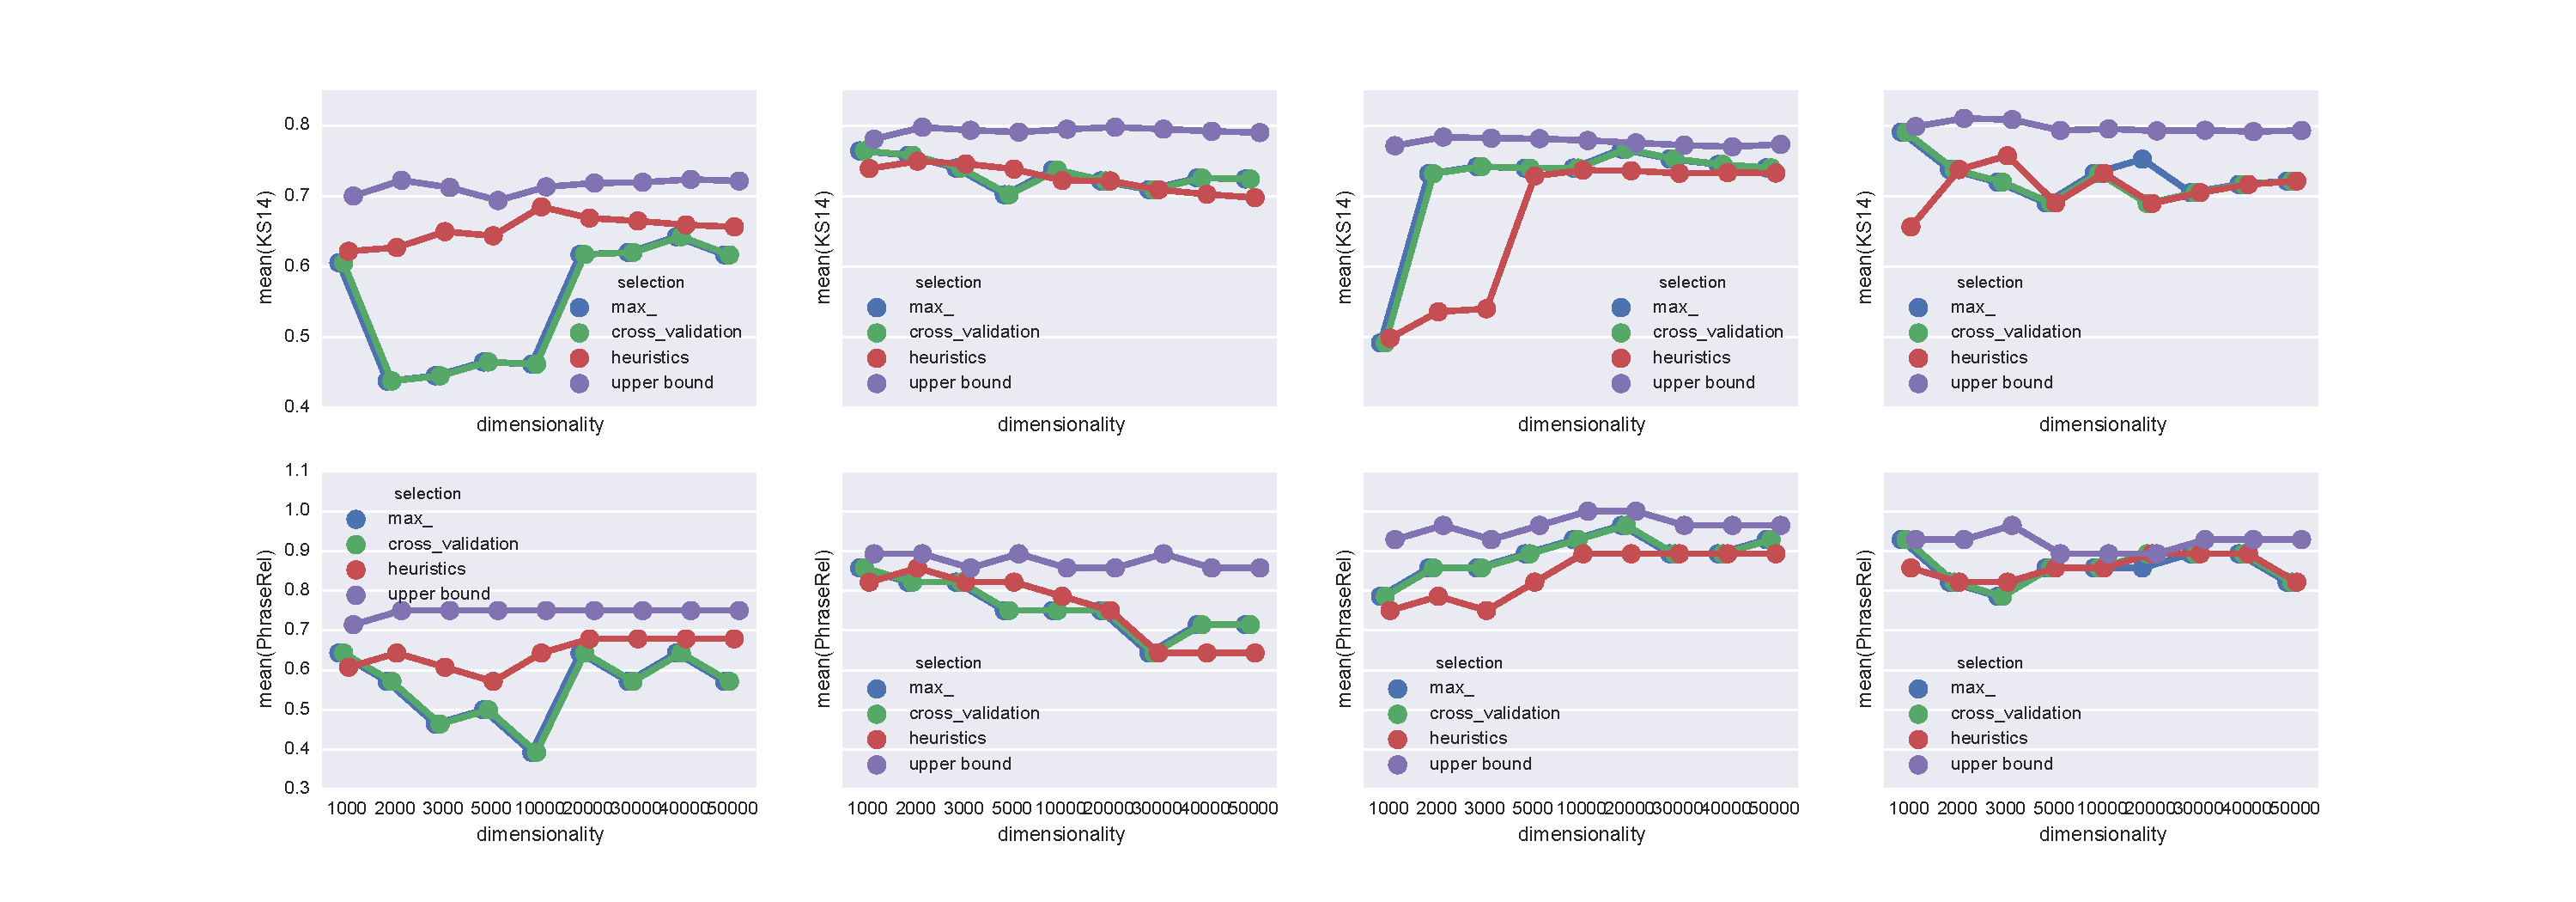
\includegraphics[width=\textwidth]{supplement/figures/GS11-transfer}
    \caption{Transfer from GS11}
    \label{fig:gs11-transfer}
\end{figure}

%%% Local Variables:
%%% mode: latex
%%% TeX-master: "../thesis"
%%% End:


Figure~\ref{fig:gs11-transfer} shows that there is little difference between Max and heuristic-based selections. In the case of \texttt{head} composition, heuristics lead to higher performance, while for low-dimensional multiplicative models heuristics fall behind the Max selection on the KS14 dataset.

% \todo[noline]{Significance tests}
When GS11 models are transferred to KS14, the average difference with the upper bound is 0.119 and 0.106 for Max and heuristics respectively. For the transfer to PhraseRel, the differences are 0.133 for Max and 0.188 for heuristics. Again, the heuristic-based selection outperforms the Max based. This supports H\ref{hyp:overfitting} that Max selection overfits, but the results are beyond the 10\% limit of H\ref{hyp:10percent}.

\subsection{Model transfer from PhraseRel}
\label{sec:from-phraserel}

\begin{figure}
  \centering
    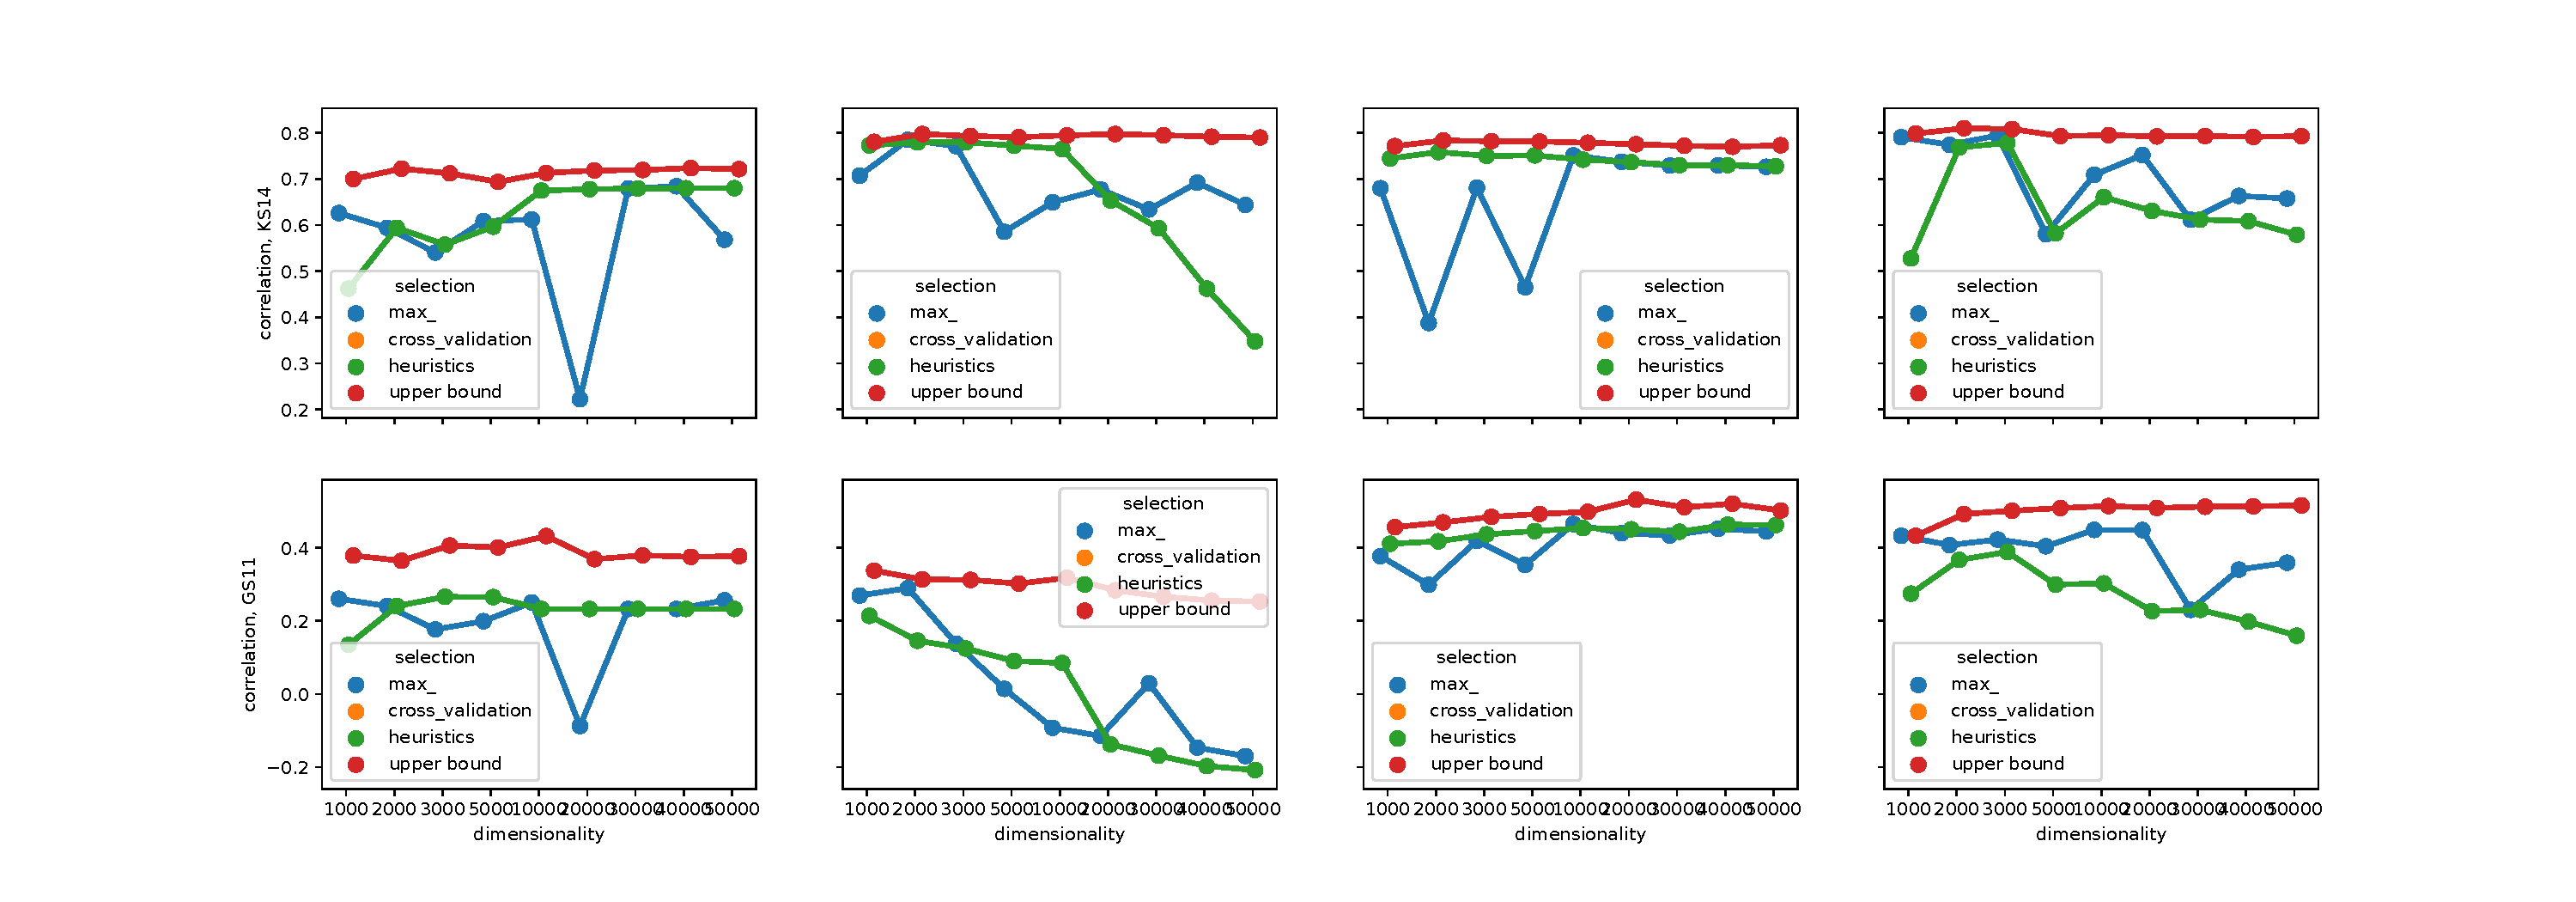
\includegraphics[width=\textwidth]{supplement/figures/PhraseRel-transfer}
    \caption{Transfer from Phraserel.}
    \label{fig:phraserel-transfer}
\end{figure}

%%% Local Variables:
%%% mode: latex
%%% TeX-master: "../thesis"
%%% End:


Figure~\ref{fig:phraserel-transfer} shows that the performance of models based on PhraseRel is less stable, especially for selection by maximum performance.

% \todo[noline]{Significance tests}
Transfer to KS14 yields the average differences of 0.152 for Max and 0.136 for heuristics. Transfer to GS11 yields the average differences of 0.454 for Max and 0.509 for heuristics. Note that the transfer from PhraseRel to GS11 is the only case where Max selection, on average, is better than heuristics.

In general, over all compositional datasets, we see---in contrast to the lexical evaluation---that the Max-based selection might be prone to overfitting (H\ref{hyp:overfitting}). However, the result difference is far beyond the 10\% limit set by H\ref{hyp:10percent}, which might be due to the different nature of the tasks: similarity, disambiguation and relevance (compositional) versus similarity and relatedness (lexical).

\section{Universal parameter selection for compositional datasets}
\label{sec:robust-param-comp-selecion}

To find parameters that are good for all three tasks, we combine their scores. As with lexical tasks, we normalise the scores on each dataset and report the average performance. The combined score is calculated the following way:

{
\scriptsize
\begin{align}
\operatorname{score}_\mathit{compositional}&(\mathit{m}, \mathit{o}) =
&\frac{1}{3}\times%
\frac{\operatorname{score}_\mathit{KS14}(\mathit{m}, \mathit{o})}%
{\max_m\operatorname{score}_\mathit{KS14}(m, \mathit{o})}%
+%
\frac{1}{3}\times%
\frac{\operatorname{score}_\mathit{GS11}(\mathit{m}, \mathit{o})}%
{\max_m\operatorname{score}_\mathit{GS11}(m, \mathit{o})}%
+%
\frac{1}{3}\times%
\frac{\operatorname{score}_\mathit{PhraseRel}(\mathit{m, \mathit{o}})}%
{\max_m\operatorname{score}_\mathit{PhraseRel}(m, \mathit{o})}%
\end{align}
%\normalsize
}
where $m$ is a model and $o$ is an operator.

Figure~\ref{fig:compositional-results} shows the performance of the models based on the combined selection over the KS14, GS11 and PhraseRel datasets. 

The performance of selected models together with the selected parameters is shown in Table~\ref{tab:compositional-max-selection} (Max selection) and Table~\ref{tab:compositional-heuristics-selection} (selection based on heuristics).

\subsection{Max selection}
\label{sec:max-selection-compositional}

Models with many dimensions do not always perform better than their low-dimensional counterparts. Particularly, only \texttt{head} and multiplication benefit from the high number of dimensions. Addition and Kronecker are closer to the upper bound with dimensionality of a few thousand.

Regarding the hypotheses, there is support of H\ref{hyp:freq} (non-constant frequency should be used with high-dimensional spaces) for addition, multiplication and Kronecker, H\ref{hyp:cds} (context distribution smoothing is optimal for high-dimensional spaces) for multiplication and H\ref{hyp:neg} (low-dimensional spaces should be dense, high-dimensional---sparse) for Kronecker.

\subsection{Heuristics}
\label{sec:heuristics-compositional}

\begin{wraptable}[6]{O}{0.5\textwidth}
% \begin{table}
  \vspace{-5em}
  \centering

  \begin{tabular}{lr}
\toprule
      parameter &  partial $R^2$ \\
\midrule
            neg &           0.40 \\
           freq &           0.29 \\
       operator &           0.21 \\
            cds &           0.15 \\
     similarity &           0.08 \\
          discr &           0.06 \\
 dimensionality &           0.05 \\
\bottomrule
\end{tabular}


  \caption{Compositional feature ablation}
  \label{tab:compositional-ablation}
\end{wraptable}


The linear model achieves  $R^2 = 0.769$. Table~\ref{tab:compositional-ablation} shows the partial $R^2$ values for the parameters. The most influential parameters are \texttt{neg}, \texttt{freq} and compositional operator.

\subsubsection{Neg}
\label{sec:neg-compositional}

For the baseline operator \texttt{head} and models with $D < 10\,000$, the \texttt{neg} should be set to 1, otherwise, it should be 1.4 (Figure~\ref{fig:compositional-neg}).

For addition, 1 is the best choice of \texttt{neg}, but the performance of $k$ values follows H\ref{hyp:neg}: the more dimensions a model has, the sparser it should be.

Multiplication benefits from denser spaces. If the dimensionality is less than 10\,000, then \texttt{neg} should be set to 0.5, otherwise 0.7 is a good choice, confirming H\ref{hyp:neg}.

Kronecker benefits from the \texttt{neg} of 0.7 if $D < 10\,000$ and from 1 for the more dimensional cases, also supporting H\ref{hyp:neg}. This is similar to multiplication, but Kronecker prefers less dense vectors.

\begin{figure}
% \begin{wrapfigure}{O}{0.5\textwidth}
  % \vspace{-30pt}
  \centering

  \begin{subfigure}[t]{\textwidth}
    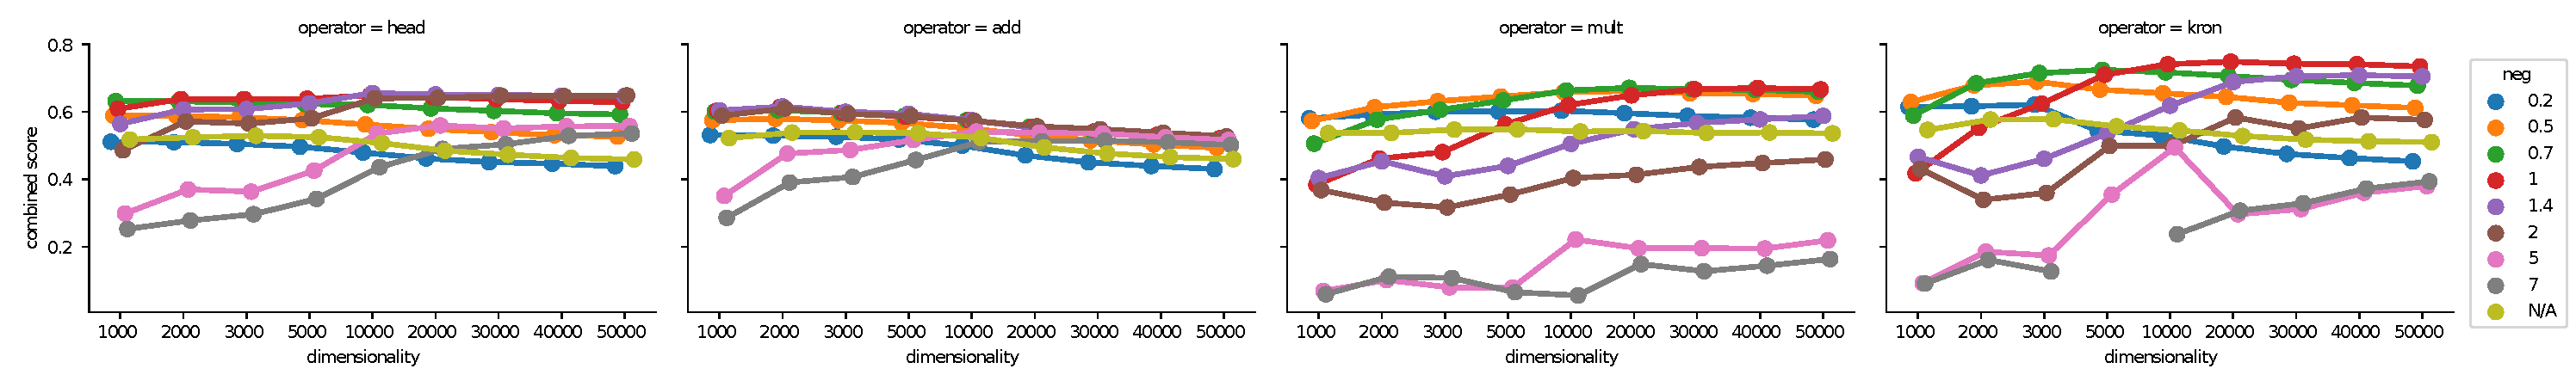
\includegraphics[width=1.1\textwidth]{supplement/figures/compositional-interaction-neg}

  \caption{\texttt{neg}}
  \label{fig:compositional-neg}
  \end{subfigure}

  \begin{subfigure}[t]{\textwidth}
    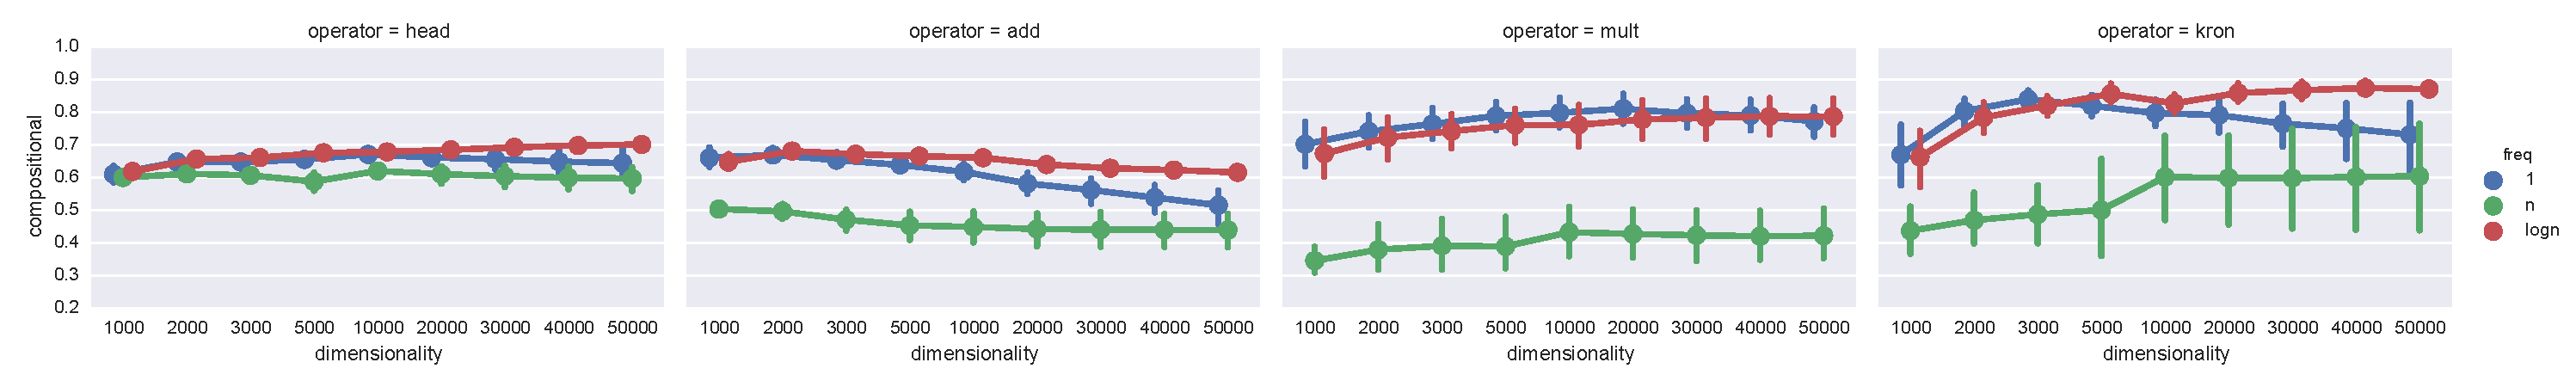
\includegraphics[width=1.1\textwidth]{supplement/figures/compositional-interaction-freq}

  \caption{\texttt{freq}}
  \label{fig:compositional-freq}
  \end{subfigure}

  \caption{Compositional.}
\end{figure}


\subsubsection{Freq}
\label{sec:freq-compositional}

The frequency value of choice of all operators is $\log n$ with an exception of multiplication, where the constant frequency is preferred (Figure~\ref{fig:compositional-freq}).

For low-dimensional vector spaces ($D \leq 5\,000$), 1 behaves well, giving support of H\ref{hyp:freq} that non-constant frequency is needed only with high-dimensional spaces.

\subsubsection{Context distribution smoothing}
\label{sec:cont-distr-smooth-compositional}

As Figure~\ref{fig:compositional-cds} shows, global context probability is the preferred choice of context probability in all cases, with an exception of Kronecker with $D > 3\,000$, where smoothed, local probabilities are better ($\alpha = 0.75$), supporting H\ref{hyp:cds} that context distribution smoothing should be used with high-dimensional spaces.

\subsubsection{Similarity}
\label{sec:similarity-compositional}

Correlation is the dominant choice of the similarity measure (Figure~\ref{fig:compositional-similarity}). However, cosine is preferred in the case of \texttt{head}, with $D > 5\,000$, and inner product is the only choice for composition with Kronecker with $D > 3\,000$.

There is no distinction between cosine and correlation for all compositional operators, which neither supports nor disputes H\ref{hyp:similarity} that expects correlation to outperform cosine with high-dimensional spaces.

\subsubsection{Discr}
\label{sec:discr-compositional}

\begin{figure}[b]
% \begin{wrapfigure}{O}{0.5\textwidth}
  % \vspace{-30pt}
  \centering

  \begin{subfigure}[t]{\textwidth}
    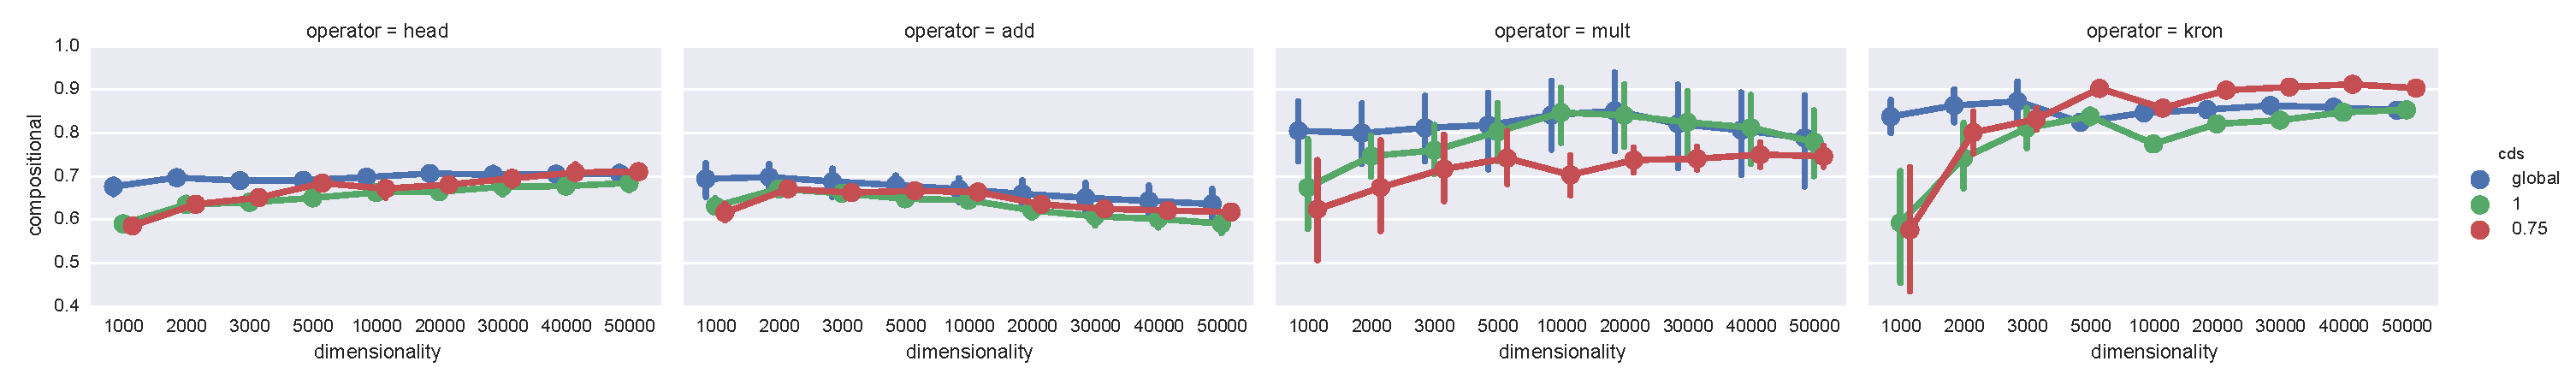
\includegraphics[width=1.1\textwidth]{supplement/figures/compositional-interaction-cds}

  \caption{\texttt{cds}}
  \label{fig:compositional-cds}
  \end{subfigure}

  \begin{subfigure}[t]{\textwidth}
    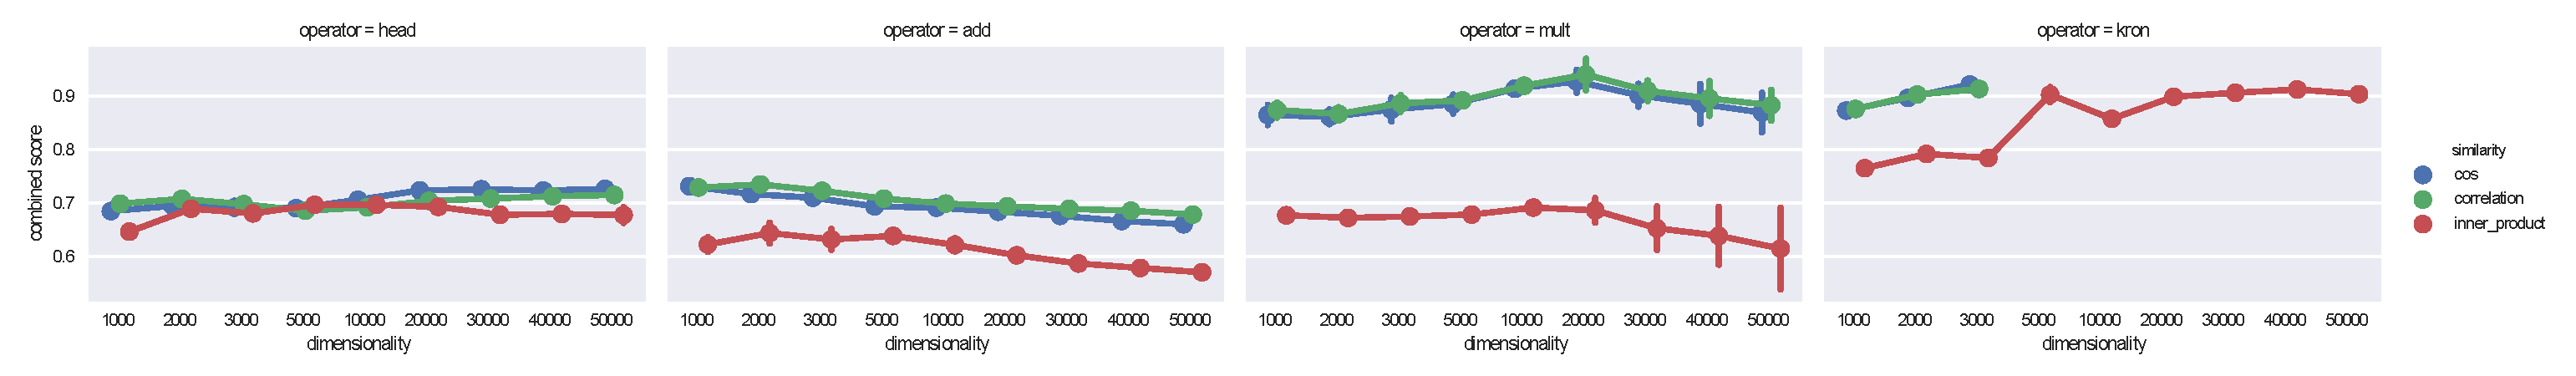
\includegraphics[width=1.1\textwidth]{supplement/figures/compositional-interaction-similarity}

  \caption{Similarity}
  \label{fig:compositional-similarity}
  \end{subfigure}

  \caption{Compositional influence of \texttt{cds} and similarity}
\end{figure}


\begin{figure}
% \begin{wrapfigure}{O}{0.5\textwidth}
  % \vspace{-30pt}
  \centering

  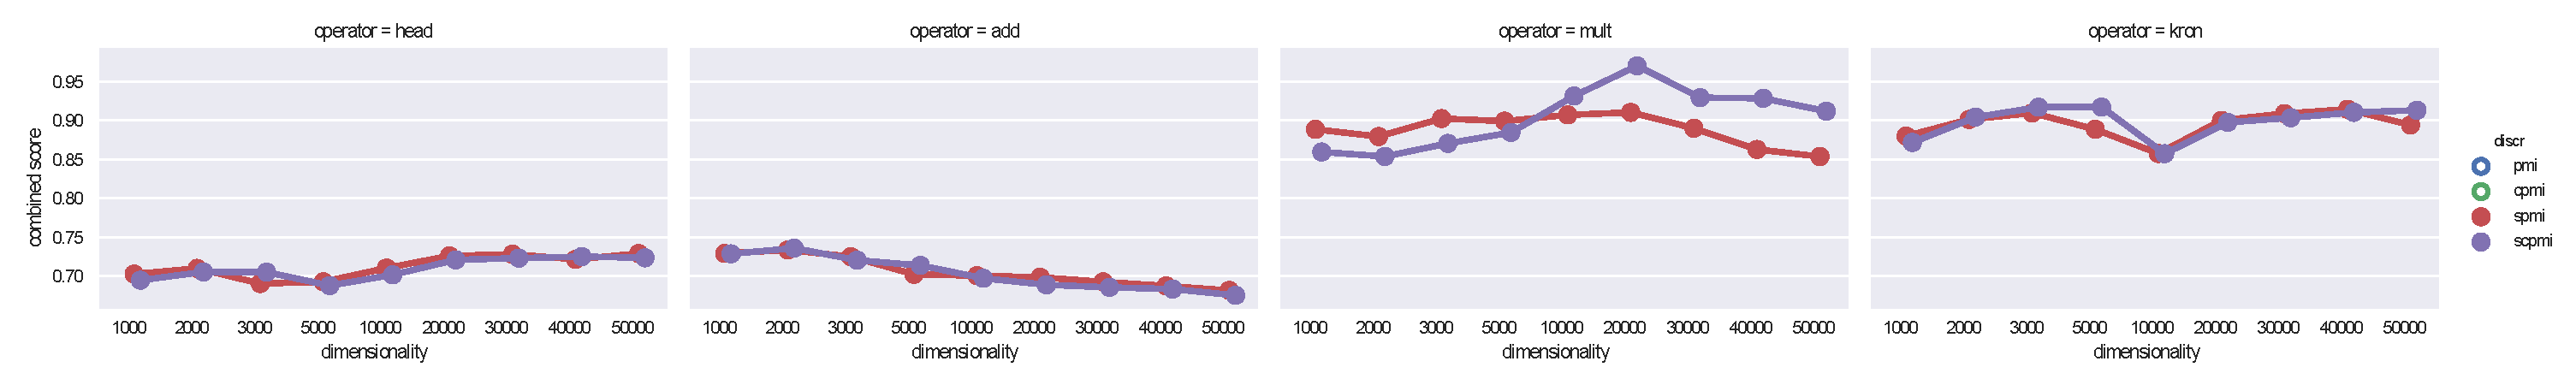
\includegraphics[width=1.1\textwidth]{supplement/figures/compositional-interaction-discr}

  \caption{Compositional influence of \texttt{discr}}
  \label{fig:compositional-discr}
\end{figure}


SPMI is the choice of \texttt{discr} that leads to the best average performance in most cases (Figure~\ref{fig:compositional-discr}). However, the difference between SPMI and SCPMI is very small.

The exceptions are Multiplicative composition with $D \geq 10\,000$ and Kronecker with $D \leq 5\,000$ where SCPMI outperforms SPMI, as expected by H\ref{hyp:comp-pmi-cpmi} that PMI values compression is needed for composition.

\subsection{Comparison with the selection based on one dataset}
\label{sec:comp-with-single-comp}

Manual selection based on a combination of the compositional datasets is more stable with regards to the chosen parameter values than the selection based on the highest values, even though manual selection does not always achieve the performance of Max selection, see Figure~\ref{fig:compositional-results}.

The average difference with the upper bound is 0.040 and 0.041 for Max and heuristics, respectively, when applied to KS14. For GS11, the difference is 0.045 (Max) and 0.127 (Heuristics). For PhraseRel, the difference is 0.055 (Max) and 0.084 (Heuristics).

The numbers are much lower than the transfer of spaces selected on the basis of one dataset (Section~\ref{sec:select-model-transf-comp}). The average normalised difference is within the 10\% limit (H\ref{hyp:10percent}), with an exception of heuristics on GS11. This is evidence that there might be one universal model that fits various tasks (H\ref{hyp:universal}). The fact that the average normalised difference is smaller for Max-based selection is against H\ref{hyp:overfitting} that expects Max selection to overfit. A combination of datasets that covers several phenomena (in our case, similarity, disambiguation and relatedness) might be more effective than manual heuristic-based selection.

The model selection procedures improve from the combination of datasets. One needs to keep in mind that in this case, we test model performance on the same dataset as we do parameter selection.

\section{Conclusion}
\label{sec:conclusion-comp}

Phrasal experiments support most of the hypotheses stated in
Section~\ref{sec:hypotheses}.

We see the confirmation of hypotheses on optimal parameter dependence on dimensionality (H\ref{hyp:dimen}). In particular: H\ref{hyp:freq} (non-constant frequency is beneficial with high-dimensional spaces) and H\ref{hyp:neg} (high-dimensional spaces should be sparser). They are supported by all datasets and confirm H\ref{hyp:dimen}. It is worth noting that even though an optimal choice of context distribution smoothing does not depend on dimensionality on KS14 and GS11, in the combined case the dependence holds.

Models that are selected on the experiments on a single dataset are prone to overfitting. Neither manual selection of parameters prevents it and the average normalised difference is above 10\% on model transfer. This confirms H\ref{hyp:overfitting} that Max selection overfits and rejects H\ref{hyp:10percent} that the relative gap in performance of the best model and a manually selected model is within 10\%.

Model selection based on the combination of datasets performs much better on each dataset (contrary to a single-dataset selected models). Both selection methods are within 10\%, supporting H\ref{hyp:10percent}.

Max selection models outperform heuristic selection models, suggesting that there is no overfitting in this case and H\ref{hyp:overfitting} is not valid. In this case, the dataset combination covered three phenomena (similarity, disambiguation and relevance) and the precaution of overfitting by heuristics might be redundant.

This also suggests that there is a unique parameter choice that is universally applicable to compositional tasks (H\ref{hyp:universal}). The universal spaces are studied in Chapter~\ref{sec:universal-param-selection}.

\chapter[Universal models]{Universal models for both lexical and compositional tasks}
\label{sec:universal-param-selection}

\lettrine[lines=5,loversize=0.25]{P}{reviously}, we identified good models for specific datasets or task types: lexical and compositional. We managed to identify models that are good for either lexical tasks or compositional. This chapter investigates how well one model can perform on all tasks in contrast to the task-tailored models of previous chapters.

This is achieved by performing the evaluation on a combined score over the previous two lexical and three phrasal datasets. We not only combine the datasets together but also look for parameters that are good across all datasets with all compositional operators. Once optimal parameters are identified, they are tested on categorical compositional methods.

Even though the identified parameters have to compromise over different tasks (lexical and compositional) and compositional methods we achieve the new state-of-the-art results with Kronecker on KS14 and GS11. Moreover, the selected lexical representations improve over the results of the categorical compositional methods reported in the literature.

\section{Operator-dependent universal models}
\label{sec:model-selection}

First, we compute combined performance scores for the following operators: head, addition, multiplication and Kronecker. We normalise the scores of every dataset and weight lexical and compositional datasets equally. Within a dataset category, the datasets are weighted equally. Such a weighting scheme is still simple, it treats the task types equally and does not focus on a particular dataset.

The combined score for a model and an operator is computed as:

{\scriptsize
  \begin{align}
    \begin{split}
\operatorname{score}_\mathit{universal}(\mathit{m}, \mathit{o}) = & %
\frac{1}{2}\times\left(
\frac{1}{2}\times%
\frac{\operatorname{score}_\mathit{SimLex-999}(\mathit{m})}%
{\max_m\operatorname{score}_\mathit{SimLex-999}(m)}%
+%
\frac{1}{2}\times%
\frac{\operatorname{score}_\mathit{MEN}(\mathit{m})}%
{\max_m\operatorname{score}_\mathit{MEN}(m)}%
\right) +
\\
&\frac{1}{2}\times\left(
\frac{1}{3}\times%
\frac{\operatorname{score}_\mathit{KS14}(\mathit{m}, \mathit{o})}%
{\max_m\operatorname{score}_\mathit{KS14}(m, \mathit{o})}%
+%
\frac{1}{3}\times%
\frac{\operatorname{score}_\mathit{GS11}(\mathit{m}, \mathit{o})}%
{\max_m\operatorname{score}_\mathit{GS11}(m, \mathit{o})}%
+%
\frac{1}{3}\times%
\frac{\operatorname{score}_\mathit{PhraseRel}(\mathit{m, \mathit{o}})}%
{\max_m\operatorname{score}_\mathit{PhraseRel}(m, \mathit{o})}%
\right)
\end{split}
\end{align}
% \normalsize
}
where $m$ stands for a model and $o$ is a compositional operator.

\subsection{Max selection}
\label{sec:max-selection-universal}

Table~\ref{tab:universal-max-selection} shows the performance of the models evaluated with a combined score of the lexical and compositional datasets.
Parameter selection is much more stable than on all previous Max-based selections. The dominant \texttt{freq} choice is $\log n$, cosine is the measure of choice for multiplication and Kronecker (if available). Correlation is the best similarity measure for the additive composition. The optimal choice of a similarity measure does not depend on dimensionality---this observation does not support H\ref{hyp:similarity} that expects such dependence.

Interestingly, when shifting is applied, dense spaces perform better: 1 and 0.7 are the optimal \texttt{neg} values. Multiplication supports H\ref{hyp:neg} that high-dimensional spaces optimally perform with sparse models.

\begin{wraptable}[6]{O}{0.5\textwidth}
  \vspace{-7em}
  \centering

  \begin{tabular}{lr}
\toprule
      parameter &  partial $R^2$ \\
\midrule
           freq &       0.32 \\
            neg &       0.29 \\
     similarity &       0.22 \\
            cds &       0.10 \\
          discr &       0.09 \\
 dimensionality &       0.07 \\
       operator &       0.05 \\
\bottomrule
\end{tabular}


  \caption{Universal (operator dependent) feature ablation}
  \label{tab:universal-ablation}
\end{wraptable}


% \todo[noline]{This is one of the major findings.}
The preference of a compositional operator depends on a model. Addition with many dimensions gives the best results on lexical tasks: 0.384 on SimLex-999 and 0.761 on MEN. Kronecker, on the other side, gives the highest values on compositional datasets supporting H\ref{hyp:order} (the word order is important for compositional operators): 0.798 on KS14, 0.514 on GS11 and 0.964 on PhraseRel. Multiplication, however, is a good compromise between the two. It gives the highest ``combined'' score of 0.945.

\subsection{Heuristics}
\label{sec:heuristics-universal}

Performance of the models selected manually is shown in Table~\ref{tab:universal-heuristics-selection}. Again, there is a lot of consistency between parameters. The linear model achieves $R^2 = 0.828$. The most influencing parameters are \texttt{freq}, \texttt{neg} and a similarity measure. See Table~\ref{tab:universal-ablation} for more details.

Heuristics for addition choose models that score the highest on lexical tasks: 0.384 on SimLex-999 and 0.764 on MEN (Table~\ref{tab:universal-heuristics-selection}). Moreover, with more than 20\,000 dimensions, there is no difference between the selection procedures (Max or heuristics) of the additive and Kronecker-based models.

Kronecker is strong in compositional tasks scoring 0.795 on KS14, 0.516 on GS11 and 0.929 on PhraseRel, which is in line with H\ref{hyp:order} that word order is important (Table~\ref{tab:universal-heuristics-selection}).

Multiplication and Kronecker support H\ref{hyp:neg}: the optimal shifting value $k$ depends on the dimensionality. Addition and Kronecker are consistent with H\ref{hyp:cds}: low-dimensional spaces benefit from global context probabilities, while high-dimensional spaces benefit from smoothed context probabilities with $\alpha=0.75$.

Multiplication, again, is a compromise between the two: it gives the highest combined score of 0.941. The highest Kronecker's combined score is 0.913, while addition's highest score is only 0.843.

Regarding the hypotheses, we clearly see on Figure~\ref{fig:universal-freq} that there is little difference between 1 and $\log n$ frequencies for the low-dimensional spaces, but $\log n$ is the best choice for the high-dimensional spaces, which is consistent with H\ref{hyp:freq}.

Shifting performs also in accordance with H\ref{hyp:neg}: for low-dimensional spaces $k=0.7$ or even $k=0.5$ leads to the highest result, while for high-dimensional spaces $k=1$ or $k=1.4$ are optimal.

We also see that there is no difference between the cosine and correlation similarity measures giving a weak support of H\ref{hyp:similarity} that correlation is optimal for high-dimensional models.

Addition and Kronecker work best with global context probabilities on low-dimensional spaces, but benefit from local probabilities ($\alpha=0.75$) for high-dimensional spaces, supporting H\ref{hyp:cds}: context distribution smoothing is beneficial with high-dimensional spaces. Multiplication, however, does not follow H\ref{hyp:cds}, as $\alpha=0.75$ leads to weak performance for all dimensions.

There is no support of H\ref{hyp:comp-pmi-cpmi}: for all operators, there is little difference between SPMI and SCPMI, so compression of PMI values might not, in general, boost the performance of compositional models.

\subsection{Comparison of the selection methods}
\label{sec:comparison-universal}

On lexical tasks, there is little difference between the model selection methods, especially for spaces with more than 30\,000 dimensions, as Figures~\ref{fig:universal-results-simlex} and \ref{fig:universal-results-men} show.

The average relative differences for Max selection are 0.034 (SimLex-999), 0.010 (MEN), 0.033 (KS14), 0.109 (GS11) and 0.061 (PhraseRel). For manual heuristics, the differences are 0.047 (SimLex-999), 0.009 (MEN), 0.034 (KS14), 0.114 (GS11) and 0.065 (PhraseRel). The numbers between different selection methods are close, with the exceptions of SimLex-999 (where Max selection is 0.013 points lower), and GS11 (where Max is lower by 0.05 points).

The high relative difference on GS11 is due to a poor performance of addition and \texttt{head}. The average normalised difference for addition is 0.219 for Max selection and 0.224 for heuristics. For the baseline compositional operator \texttt{head}, the differences are 0.105 and 0.141 respectively. The differences for multiplication and Kronecker are less than 0.07, which is in accordance with the 10\% margin of H\ref{hyp:10percent}.

Contrary to H\ref{hyp:overfitting}, Max selection does not overfit, probably due to a broad selection of evaluation datasets.

% \todo[noline]{One of the major findings.}
When the models that are selected on lexical tasks are applied in a compositional setting, they perform worse than the models selected based on the universal score. This suggests that a model that is good for lexical tasks will not necessarily perform well on a compositional task, rejecting H\ref{hyp:not-lextocomp}.

In addition, the difference between the good lexical models and the upper bound increases as dimensionality increases. This is the case for multiplication, the most notable difference is observed on KS14 (Figure~\ref{fig:universal-results-ks14}).

It worth noting that on compositional tasks dimensionality does not contribute as much as on lexical tasks, with an exception of addition on the GS11 dataset, where performance decreases as dimensionality increases.

\section{An operator-independent universal model}
\label{sec:single}

In the previous section, we have seen that even though parameter selection varies between operators, there are parameter choices that are shared, for example, correlation is the best similarity measure for addition, multiplication and Kronecker (if $D \le 3\,000$). Given this and the fact that the difference between some of the choices is marginal, we try to look for a truly universal parameter combination. The aggregated score of a model is computed as:

{\scriptsize
\begin{align}
  \begin{split}
\operatorname{score}_\mathit{universal}(\mathit{m}) = &%
\frac{1}{2}\left(
\frac{1}{2}%
\frac{\operatorname{score}_\mathit{SimLex-999}(\mathit{m})}%
{\max_m\operatorname{score}_\mathit{SimLex-999}(m)}%
+%
\frac{1}{2}%
\frac{\operatorname{score}_\mathit{MEN}(\mathit{m})}%
{\max_m\operatorname{score}_\mathit{MEN}(m)}%
\right)+
\\
&\frac{1}{2}\Bigg(
\frac{1}{6}%
\frac{\operatorname{score}_\mathit{KS14}(\mathit{m}, \mathit{add})}%
{\max_m\operatorname{score}_\mathit{KS14}(m, \mathit{add})}%
+%
\frac{1}{6}%
\frac{\operatorname{score}_\mathit{GS11}(\mathit{m}, \mathit{add})}%
{\max_m\operatorname{score}_\mathit{GS11}(m, \mathit{add})}%
+%
\frac{1}{6}%
\frac{\operatorname{score}_\mathit{PhraseRel}(\mathit{m, \mathit{add}})}%
{\max_m\operatorname{score}_\mathit{PhraseRel}(m, \mathit{add})}
+
\\
&\phantom{\frac{1}{2}\Bigg(}
\frac{1}{6}%
\frac{\operatorname{score}_\mathit{KS14}(\mathit{m}, \mathit{mult})}%
{\max_m\operatorname{score}_\mathit{KS14}(m, \mathit{mult})}%
+%
\frac{1}{6}%
\frac{\operatorname{score}_\mathit{GS11}(\mathit{m}, \mathit{mult})}%
{\max_m\operatorname{score}_\mathit{GS11}(m, \mathit{mult})}%
+%
\frac{1}{6}%
\frac{\operatorname{score}_\mathit{PhraseRel}(\mathit{m, \mathit{mult}})}%
{\max_m\operatorname{score}_\mathit{PhraseRel}(m, \mathit{mult})}
\Bigg)
\end{split}
\end{align}
\normalsize
}
where $\mathit{add}$ stands for addition and $\mathit{mult}$ stands for multiplication. We do not test Kronecker, because it is not tested on all dimensions with the cosine and correlation similarity measures. We also exclude the baseline operator \texttt{head}.

\subsection{Max selection}
\label{sec:max-selection-single}

Table~\ref{tab:single-max-selection} shows the combined scores for all datasets abstracting over a compositional operator.

The parameter selection shows a clear pattern. Low-dimensional spaces perform best with 1 as the frequency choice, while high-dimensional models perform better with $\log n$, confirming to H\ref{hyp:freq} that non-linear frequency should be used with high-dimensional models. Cosine is a better-suited similarity measure for models with few dimensions and correlation is suited to those with many, which is in line with H\ref{hyp:similarity}. Finally, global context probabilities are the best in a low-dimensional case, while local context probabilities perform best with many dimensions, supporting H\ref{hyp:cds}.

\subsection{Heuristics}
\label{sec:heuristics-single}

\begin{wraptable}[10]{O}{0.5\textwidth}
%\begin{table}[b]
  % \vspace{-2em}
  \centering

  \begin{tabular}{lr}
\toprule
      parameter &  partial $R^2$ \\
\midrule
           freq &   0.434 \\
     similarity &   0.269 \\
            neg &   0.196 \\
          discr &   0.092 \\
            cds &   0.090 \\
 dimensionality &   0.034 \\
\bottomrule
\end{tabular}


  \caption{Universal (operator-independent) feature ablation}
  \label{tab:single-ablation}
  % \end{wraptable}
\end{wraptable}


The linear model gives $R^2 = 0.898$. The most influential parameters are \texttt{freq}, similarity measure and \texttt{neg}, refer to Table~\ref{tab:single-ablation}.

Heuristics, in general, repeat the parameter choices of Max selection, but the switch between parameter values happens at a higher number of dimensions (at 20\,000, not at 5\,000). Refer to Table~\ref{tab:single-heuristics-selection} for the results and Figure~\ref{fig:single-params} for the parameter behaviour.

The average normalised differences with the upper bound for Max selection are 0.049 (SimLex-999), 0.032 (MEN), 0.063 (KS14), 0.106 (GS11) and 0.116 (PhraseRel). The differences for heuristics are in general higher: 0.062 (SimLex-999), 0.045 (MEN), 0.076 (KS14), 0.090 (GS11) and 0.139 (PhraseRel).

Max selection is above the 10\% margin of H\ref{hyp:10percent} on GS11 and PraseRel, while heuristics are above the margin only on PhraseRel.

\section{Experiments with categorical compositional operators}
\label{sec:frob-comp-oper}

Sections~\ref{sec:model-selection} and \ref{sec:single} identified models that perform well on a range of tasks. The majority of them are within the 10\% margin set by H\ref{hyp:10percent}. We apply selected models with tensor-based operators on phrasal datasets (KS14, GS11 and PhraseRel).

\begin{table}
  \centering
  \begin{tabular}{lrrr}
\toprule
Operator &   KS14 &   GS11 &  PhraseRel \\
\midrule
Add              &  0.785 &  0.338 &      0.893 \\
Mult             &  0.771 &  0.507 &      \textbf{1.000} \\
Kron             &  \textbf{0.798} &  \textbf{0.516} &      0.964 \\
Relational       &  0.768 &  0.393 &      0.893 \\
Copy-object      &  0.628 &  0.278 &      0.821 \\
Copy-subject     &  0.738 &  0.402 &      0.821 \\
Frobenius-add   &  0.761 &  0.374 &      0.821 \\
Frobenius-mult  &  0.747 &  0.299 &      0.857 \\
Frobenius-outer &  0.765 &  0.385 &      0.893 \\
\bottomrule
\end{tabular}


  \caption{The best scores on compositional tasks based on the universal selections.}
  \label{tab:frobenius-results}
\end{table}


Table~\ref{tab:frobenius-results} shows the best results we obtained for each operator, Tables~\ref{tab:frobenius-ks14-results}, \ref{tab:frobenius-gs11-results} and \ref{tab:frobenius-phraserel-results} show all the results together with the model parameters and Figure~\ref{fig:frobenius-results} depicts the data.

In general, the best results are achieved with 3\,000-dimensional models (with an exception on GS11 where 1\,000-dimensional models perform better in 4 out of 6 cases, and copy-subject on KS14). Also, performance increases as dimensionality increases.

Max selection based on Kronecker leads to the highest results. The exceptions are Frobenius multiplication and copy-subject on KS14, where the model that is best with addition also leads to the highest results among tensor-based composition. On PhraseRel, copy-subject performs best with operator-independently selected space.

Relational is the fourth best compositional operator after addition, multiplication or Kronecker on KS14 (0.768) and PhraseRel (0.893). Copy-subject is the best on GS11 (0.402). Frobenius-outer gives the highest result on PhraseRel together with relational.

On GS11 and PhraseRel, newly tested operators outperform addition, whose scores are 0.338 and 0.893, respectively.

While there is a difference between selection methods, there are no clear outliers and the models show similar behaviour.

\section{Putting results into perspective}
\label{sec:comp-with-other}

This section discusses the results of the experiments in the context of our preliminary studies and the work of others.

In an earlier study \cite{milajevs-EtAl:2014:EMNLP2014}, we compared a PPMI-weighted space, an LMI-weighted and SVD-reduced space and a space based on the original word2vec vectors obtained from the Google News corpus \cite{mikolov2013distributed}. The same compositional operators were evaluated as in this thesis. The count-based models selected in the earlier study were the ones that were considered to be efficient in the compositional tasks and were used in the studies that introduced the evaluation datasets: KS14 \cite{kartsadrqpl2014} and GS11 \cite{Grefenstette:2011:ESC:2145432.2145580}. Thus, \newcite{milajevs-EtAl:2014:EMNLP2014} can be seen as a replication of the experiments in previous papers. The experiments showed that on small-scale tasks (KS14 and GS11) count-based models are competitive with neural word vectors, however, word2vec vectors are superior in dialog act tagging and paraphrase detection.

In that study, additive composition with an SVD-reduced space gave the best result of 0.732 on KS14. The best tensor-based result was 0.655, achieved with word2vec and copy-object. All our models (Table~\ref{tab:frobenius-results}), with the exception of copy-object, improve over our previous best scores. Despite being lower, our copy-object (0.628) is close to the word2vec score reported in \newcite{milajevs-EtAl:2014:EMNLP2014}.

On the GS11 dataset, systematic parameter selection leads to spaces that improve over the corresponding operators in the earlier study on all but two of the compositional methods (the exceptions being copy-object and Frobenius mult). In addition to that, multiplication and Kronecker improve over the overall best-reported score of 0.456 in \newcite{milajevs-EtAl:2014:EMNLP2014}. Kronecker yields the highest score of 0.516.

\newcite{kim2015neural} adopt the evaluation procedure of \newcite{milajevs-EtAl:2014:EMNLP2014} to test an extended word2vec model that is tuned for multiplicative interaction of the vectors, not additive, as the original word2vec. They improve on most of the composition operators on the KS14 and GS11 datasets.

They achieve the best result of 0.770 with addition on KS14. Three of our models (addition, multiplication and Kronecker) outperform that score. Also, our results are better than the results reported  by comparing results by operator (our result are shown in brackets for comparison): multiplication 0.440 (0.771), Kronecker 0.623 (0.798), relational 0.665 (0.768), copy-subject 0.454 (0.738), copy-object 0.607 (0.628), Frobenius addition 0.610 (0.761), Frobenius multiplication 0.608 (0.747), Frobenius outer 0.664 (0.765).

On G11, their best score is 0.387, which is lower than the results that we get with multiplication, Kronecker, relational and copy-subject. However, we get lower results with copy-object and Frobenius outer.

\newcite{hashimoto-tsuruoka:2015:CVSC} learn the matrices of transitive verbs using implicit tensor factorisation. The verb matrices are learned in two ways: one only takes into account the verb arguments (the subject and the object, referred as SVO in the paper), another, in addition to that, employs the adjuncts that complement the meaning of the verb phrases (SVOPN). They use copy-subject as the compositional operator. The main baseline is their previous method described in \newcite{hashimoto-EtAl:2014:EMNLP2014}.

In comparison to their SVO results, our are higher: they get 0.480 on GS11 and 0.481 on KS14. These results are lower than our Multiplication and Kronecker on GS11 and all operators on KS14.

The SVOPN model with the score of 0.614 outperforms our best (0.516) on GS11. While they get a higher score on KS14 of 0.744 (though it is obtained with the \newcite{hashimoto-EtAl:2014:EMNLP2014} baseline) it is still lower than all of our results, except copy-subject and copy-object. Interestingly, our result of 0.738 with copy-subject is close to their score but is still lower.

\newcite{hashimoto-tsuruoka:2016:P16-1} jointly learn compositional and non-compositional phrase embeddings by using a compositionality scoring function. They improve on their previous work and get the score of 0.680 on GS11 versus our 0.516.

\newcite{fried-polajnar-clark:2015:ACL-IJCNLP} use low-rank tensors to approximate third-order tensors of verbs. They achieve the scores of 0.47 on GS11 and 0.68 on KS14 with categorical composition and 0.71 on KS14 with addition. While our best result is higher on GS11, categorical operators score lower, the best is copy-subject (0.402). On KS14, our experiments produce higher results (with an exception of copy-object) than their best (additive) model. It is worth noting the study of \newcite{polajnar-rimell-clark:2015:LSDSem} uses discourse features to build vectors, but the experiment results reported there are not compatible with ours because we averaged the human-provided scores before computing correlation, while they treat each human score individually without averaging.

Overall, we improved over the scores by identifying a better set of model parameters rather than developing a more sophisticated model.

\section{Conclusion}
\label{sec:conclusion-universal}

This chapter identified a few spaces that work well on a broad range of lexical and compositional tasks.

Despite the expectation in H\ref{hyp:overfitting}, we see that Max selection does not overfit if the models are evaluated on diverse tasks. In fact, heuristics become too conservative in this case, however, we still suggest manual analysis when a small number of datasets is used.

Our universal models perform within the 10\% margin of H\ref{hyp:10percent} in the majority of the experiments. Moreover, the operator-independent universal space is competitive with spaces that were selected with an operator in mind, supporting the idea that there is a universal vector space for all kind of tasks and H\ref{hyp:universal}.

The selections show that an optimal parameter choice depends on dimensionality (H\ref{hyp:dimen}). As we have seen in Section~\ref{sec:comparison-universal}, a good lexical model might fail in a compositional setting (H\ref{hyp:not-lextocomp}). We have also seen in Section~\ref{sec:max-selection-universal} that good lexical models favour the additive composition, while Kronecker is more optimal for composition and multiplication is a compromise between the two. This, and the fact that a similarity has been found between lexical and compositional tasks \cite[\textcolor{citecolor}{Section~4}]{kiela-clark:2014:CVSC}, might be an explanation of why addition is considered to be the best compositional operator. In our experiments, multiplication and Kronecker consistently outperform addition.

While parameter selection depends on dimensionality, the performance on compositional task depends on it to a much lower extent.

Our selection methodology has produced significantly better results in the KS14 dataset over widely used count-based vectors \cite{milajevs-EtAl:2014:EMNLP2014}, neural vectors in a compositional setting \cite{milajevs-EtAl:2014:EMNLP2014,kim2015neural} and learned verb tensors \cite{fried-polajnar-clark:2015:ACL-IJCNLP,hashimoto-tsuruoka:2016:P16-1,hashimoto-tsuruoka:2015:CVSC}.

While our results on GS11 are close to the current state-of-the-art results \cite{hashimoto-tsuruoka:2016:P16-1}, there is room for improvement, especially for tensor-based compositional operators. The difference in the performance might be explained as the limit of the count-based methods or the unexplored, and therefore untuned, parameters of the verb matrix. For example, we consider all different subject-object occurrences despite their frequency in the corpus. Using only the subject-object pairs that appeared at least 100 times might improve the results.

The gap between the multiplicative and Kronecker composition in our work indicates that the categorical methods can be improved. We see that the word order is important in the task, otherwise, Kronecker would not outperform addition and multiplication. Because categorical methods take word order into account, there is a potential for them to improve. However, it is not clear whether the verb matrices are of good quality. The verb matrices obtained by different ways need to be tested on a lexical similarity task, for example \newcite{2016arXiv160800869G}. Also, the similarity judgments of verbs in SimLex-999 and MEN can be used.



%%% Local Variables:
%%% mode: latex
%%% TeX-master: "thesis"
%%% TeX-engine: xetex
%%% End:
